\documentclass[review]{elsarticle}

\usepackage{xr} %% For cross-referencing supl figures
\externaldocument[S-]{Supplementary}

\usepackage{lineno,hyperref}
\usepackage[utf8]{inputenc}
\usepackage{graphicx}
\usepackage{amsfonts}
\usepackage{mathtools}

%% for the annex figure
\usepackage{tikz}
\usetikzlibrary{shapes,arrows,chains,calc}
% Set up a few colours for tikz figure
\colorlet{lcfree}{green}
\colorlet{lcnorm}{blue}
\colorlet{lccong}{red}

\usepackage{hhline}
\usepackage{booktabs}
\usepackage[textsize=scriptsize]{todonotes}
%\usepackage[textsize=scriptsize, disable]{todonotes}  %% to turn off notes
\usepackage{eurosym}
\usepackage{longtable}

% For track-changes
%\usepackage[draft]{changes}
\usepackage[final]{changes} %% to turn off changes
\definechangesauthor[color = red]{JM}
\definechangesauthor[color = blue]{PD}
\definechangesauthor[color = green!40!black]{JJ}
\definechangesauthor[color = purple]{CM}

\modulolinenumbers[1]

\journal{Ecological Modelling}

%% Harvard
\bibliographystyle{model2-names.bst}\biboptions{authoryear}
%%%%%%%%%%%%%%%%%%%%%%%

\begin{document}

\begin{frontmatter}
\title{\emph{MixFishSim}: highly resolved spatiotemporal simulations for
	exploring mixed fishery dynamics}

%% Group authors per affiliation:
\author[1,2]{Paul J. Dolder\corref{c}}
\cortext[c]{Corresponding author}
\ead{paul.dolder@gmit.ie}

\author[1]{Cóilín Minto}
\author[3]{Jean-Marc Guarini}
\author[4]{Jan Jaap Poos}

\address[1]{Galway-Mayo Institute of Technology (GMIT), Dublin Road, Galway,
	Ireland} 
\address[2]{Centre for Environment, Fisheries and Aquaculture Science (Cefas),
	Pakefield Road, Lowestoft, UK}
\address[3]{\replaced[id=JM]{Sorbonne Université, Faculty of
		Sciences}{Université Pierre et Marie Curie}, 4 Place Jussieu,
	75005 Paris, France}
\address[4]{Wageningen Marine Research, Haringkade 1 1976 CP IJmuiden,
	Netherlands}

\begin{abstract}

\replaced[id = JJ]{Most fisheries}{Fishing} exploit\deleted[id=JJ]{s} a variety 
of spatially and temporally heterogeneous fish populations using
species-unselective gear that can result in unintended, unwanted catch of low
quota or protected species. Reducing these unwanted catches is crucial for
biological and economic sustainability of `mixed fisheries' and implementation
of an ecosystem approach to fishing. \\

\replaced[id = PD]{If fisheries are to avoid unwanted catch}{To implement
	effective spatial measures to reduce discards} a good understanding of
spatiotemporal fishery dynamics is required. However, traditional scientific
advice is limited by a lack of highly resolved knowledge of population
distributions, population movement and how fishers interact with different fish
populations. This reflects the fact that data on fish location at high temporal
and spatial resolutions is expensive and difficult to collect. Proxies inferred
from either scientific surveys or commercial catch data are often used to model
distributions, often with sparse data at limited spatial and temporal
resolution. \\ 

To understand how data resolution impacts inference on mixed fisheries
interactions, we develop a highly resolved spatiotemporal simulation model
incorporating: i) delay-difference population dynamics, ii) population movement
using Gaussian Random Fields to simulate patchy, heterogeneously distributed
populations, and iii) fishery dynamics for multiple fleet characteristics based
on species targeting via a mix of correlated random walk movement (for
exploration) and learned behaviour (for exploitation) phases of the fisheries.
\\ 

We simulate 50 years of fishing and use the results from the fisheries catch to
draw inference on the underlying population structures. We compare this
inference to i) a simulated fixed-site sampling design commonly used for
fisheries monitoring purposes, and ii) the true underlying population
structures input to the simulation. We use the results to establish the
potential and limitations of fishery-dependent data in providing a robust
picture of spatiotemporal distributions. Finally, we simulate an area closure
based on areas defined from the known ("real-population") distribution,
commercial catch data and survey data at different temporal and spatial
resolutions and assess their effectiveness on reducing catches of a fish
population. \\

We conclude from our simulations that commercial data, while containing bias,
provides a useful tool for managing catches in mixed fisheries if applied at
the correct spatiotemporal scale. \\

[333 words]

\end{abstract}

\begin{keyword}
Some\sep keywords \sep here. Max 6 
\MSC[2010] 00-01\sep  99-00
\end{keyword}

\end{frontmatter}

\linenumbers

\section{Introduction}

Fishers exploit a variety of fish populations that are heterogeneously
distributed in space and time with varying knowledge of species distributions
using species-unselective fishing gear. \added[id=PD]{In doing so} fisheries
\deleted[id=PD]{that}catch an assemblage of species
\added[id=PD]{and}\deleted{, known as mixed fisheries} \replaced[id=JJ]{may}{,
	when managed by single-species quotas can end up}
discard\deleted[id=JJ]{ing} overquota catch \added[id=JJ]{when managed by
	single species quotas and fishers exhaust or more quota, may} lead to
overexploitation of fish populations \added[id=JJ]{\citep{Ulrich2011a,
		Batsleer2015}}.  \added[id=JJ]{This discarding of fish in
	excess of quota hampers the ability to limit fishing mortality to
	within sustainable limits \citep{Alverson1994, Crowder1998,
		Rijnsdorp2007}} \deleted[id=PD]{; reducing discarding is
	crucial}and the ability to manage for the biological and economic
sustainability of fisheries\deleted[id=JJ]{ and implementation of an ecosystem
	approach to fisheries}. As such, there is increasing interest in
technical solutions such as gear and spatial closures as ways of
\replaced[id=PD]{reducing unwanted catch}{avoiding discard\added[id=JJ]{ing of
		fish}}\citep{Kennelly2002, Catchpole2008, Bellido2011}.  \\

\replaced[id=PD]{Changes to spatial fishing patterns have}{Use of spatial
	management as a tools} been proposed as a method to reduce discards
\added[id=PD]{\citep{Holmes2011, Little2014, Dunn2014a}}. However,
\deleted[id=PD]{its} implementation of avoidance measures is hampered by lack
of knowledge of fish and fishery spatiotemporal dynamics and understanding of
the scale at which processes are important for management. Understanding the
correct scale for spatial measures is crucial in order to implement measures at
a resolution that ensures effective management \citep{Dunn2016} while
minimising economic impact.  For example, a scale that promotes species
avoidance for vulnerable or low quota species while allowing continuance of
sustainable fisheries for available quota species.\\

\replaced[id=PD]{Identifying}{Ensuring measures are implemented at} an
appropriate scale has been a challenge in the past that has led to ineffectual
measures with unintended consequences such as limited impact towards the
management objective or increased benthic impact on previously unexploited
areas (e.g. the cod closure in the North Sea
\citep{Rijnsdorp2001,Dinmore2003}). \replaced[id=PD]{M}{Since then m}ore
refined spatial information has \added[id=PD]{since} become available through
the combination of logbook and Vessel Monitoring System (VMS) data
\citep{Lee2010, Bastardie2010, Gerritsen2012, Mateo2016} and more real-time
spatial management has been possible \citep[e.g.][]{Holmes2011}.  However, such
information is derived from an inherently biased sampling programme, targeted
fishing. \deleted[id=PD]{ Further, fishers generally only recorded landings
	(not catch) on a daily basis\todo{\added[id=JJ]{Its not clear what the
			problem is: landings collected on daily basis or
			landings recorded rather than catch}}.  This leads to
	questions about the validity of inference that can be drawn from
	landings data assigned to VMS activity pings.}\todo{\added[id=JJ]{This
		comes as a surprise: I thought this was going to be about
		discards}\added[id=PD]{Agree, have removed this to avoid
		confusion}}\\ 

In order to understand \replaced[id=PD]{the consequences of using}{challenges
	that face} VMS-linked landings to draw inference on the underlying
population structure we develop a simulation model where population dynamics
are highly-resolved in space and time\replaced[id=PD]{. Being}{ and are}
known \added[id=PD]{directly} rather than inferred from sampling or commercial
catch\added[id=PD]{, we can use the population model to evaluate how inference from
	fisheries-dependent and fisheries independent sampling relates to the
	real population structure}. \replaced[id=PD]{In our model system
	p}{P}opulation movement is driven by random (diffusive) and directed
(advective) processes and we incorporate characterisation of a number of
different fishing \added[id=PD]{fleet dynamics} exploiting four fish populations
with different spatial and population demographics.\\

Using our model we simulate \replaced[id=PD]{50}{40} years of exploitation of
the fish populations. \replaced[id=PD]{We}{ and} use the
results\deleted[id=PD]{ from the fishing model:}

\begin{enumerate}
	\item to understand how sampling-derived data reflects the underlying
		population structures. We compare at different spatial and
		temporal aggregations of the simulated population distributions
		to: 
		\begin{enumerate}
			\item the inferred population from a stratified
				fixed-site sampling survey design commonly used
				for fisheries monitoring purposes, otherwise
				know as a fisheries-independent survey,
			\item the inferred population from our
				fishery-dependent model which includes
				fishery-induced sampling dynamics.\\
		\end{enumerate}
	\item to understand the impact of data aggregation and data source on
		spatial fisheries management measures we simulate a fishery
		closure to protect a species based on different spatial and
		temporal data aggregations:
		\begin{enumerate}
			\item as if the real spatial population structure were
				known,
			\item the fishery-independent inferred population
				structure
			\item the fishery-dependent inferred population
				structure
		\end{enumerate}
		We evaluate the theoretical "benefit" to the population of the
		closure(s), the effect on the other three populations and
		fishery catch.\todo{\added[id=JJ]{If the paper has two goals
				this should be clear from the start, but may be
				better over 2 MSs}\added[id=PD]{I would like to
				keep both parts, but have made clearer in how
				its set out. The closure scenarios form
				validation of the data aggregation, rather than
				effectiveness of the closures themselves - so
				its a continuation of the same question in my
				eyes}}\deleted[id=PD]{.  Further, we extend our
			analysis to a range of spatial and temporal scales to
			assess the impact of these processes on the success of
			the management measure.}\\
\end{enumerate}


\section{Materials and Methods}

\replaced[id=PD]{A}{We developed and implemented a simulation model with a}
modular event-based \replaced{simulation model was developed with}{approach,
	where} \added[id=PD]{sub-}modules \deleted[id=PD]{are} implemented on
independent time-scales appropriate to capture the characteristic of the
\replaced[id=PD]{different processes}{process modelled} (Figure 1).
\added[id=PD]{The following sub-modules were included to capture the full
	system: 1) Population dynamics, 2) Recruitment dynamics, 3) Population
	movement, 4) fishery dynamics.}\\

\deleted[id=PD]{The fishing model operated on a tow-by-tow basis, while}
\replaced[id=PD]{P}{p}opulation dynamics (fishing and natural mortality,
growth) operate on a daily time-step\replaced[id=PD]{, while p}{. P}opulation
movement occurs on a weekly time-step\replaced[id=PD]{. R}{, while r}ecruitment
\replaced[id=PD]{takes place}{occurs} periodcally each year for a set time
\replaced[id=PD]{duration}{period (e.g. 3 weeks)} specified for each
population\deleted[id=PD]{.}\added[id=PD]{, while the fishing module operates
	on a tow-by-tow basis (i.e. multiple events a day)}.  The simulation
framework is implemented in the statistical software package R
\citep{RCoreTeam2017} \replaced[id=PD]{and}{;} available as an R package from
the authors github site (\url{www.github.com/pdolder/MixFishSim}).\\

\deleted[id=PD]{Here we describe each of the model components; 1) Population
	dynamics, 2) Recruitment dynamics, 3) Population movement dynamics, 4)
	fishery dynamics.}

%% the tikz figure
\clearpage

%%%%%%%%%%%%%%%%%%%%%%%%%%%%%%%%%%%
% Overview schematic  
\begin{figure}[!ht]
	\hspace{-4em}
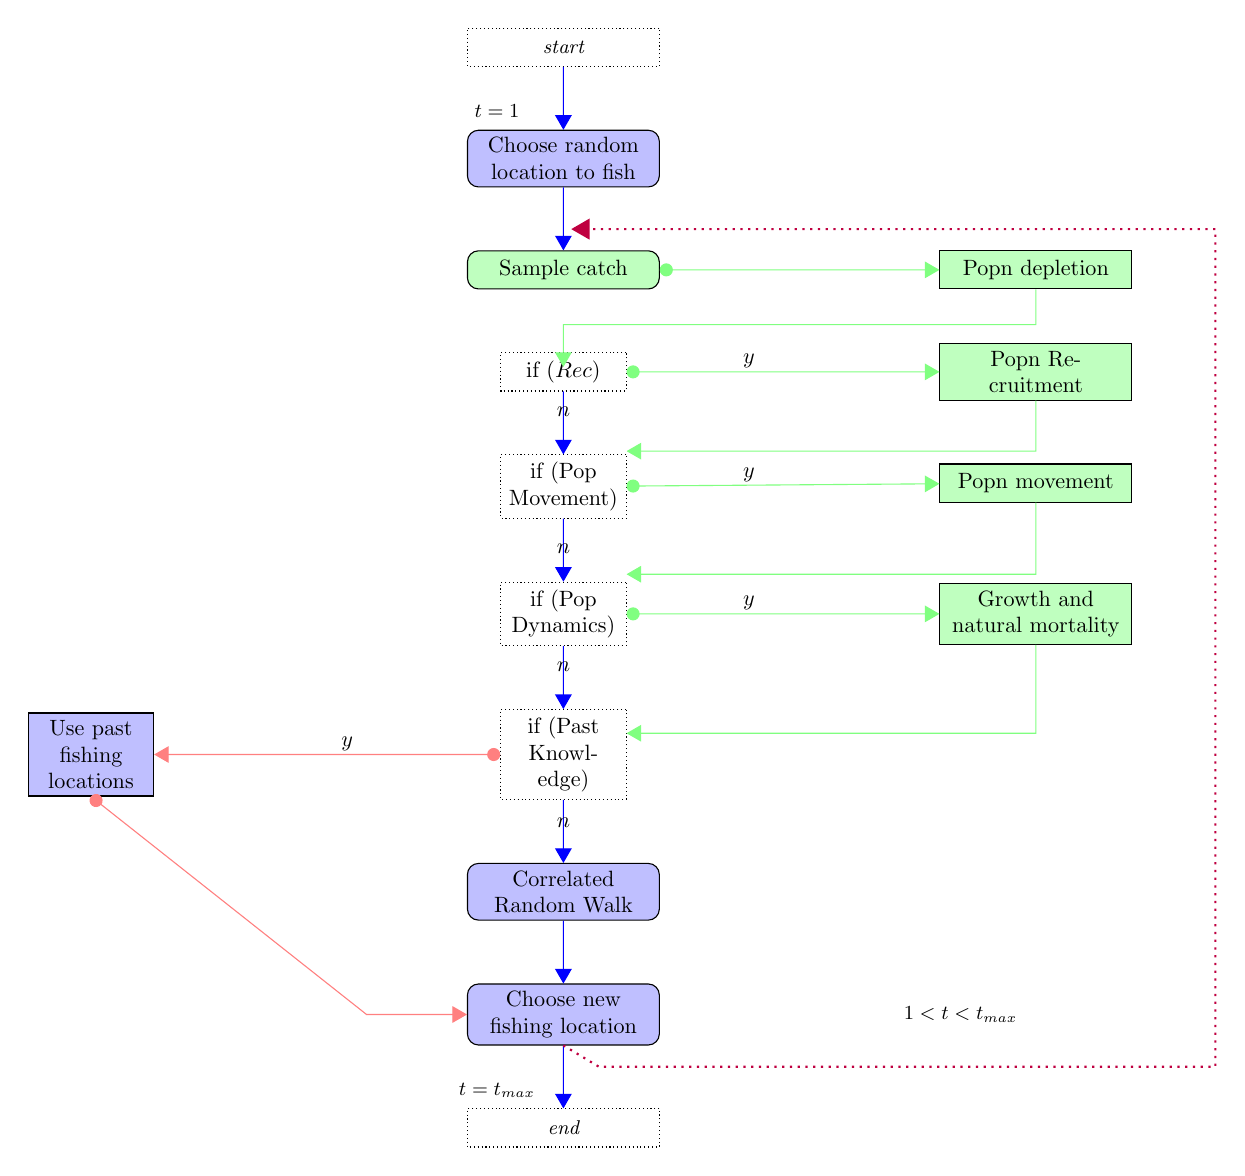
\begin{tikzpicture}[%
    >=triangle 60,              % Nice arrows; your taste may be different
    start chain=going below,    % General flow is top-to-bottom
    node distance=8mm and 60mm, % Global setup of box spacing
    every join/.style={norm},   % Default linetype for connecting boxes
    scale=0.9,
    every node/.style={scale=0.8}]                 
    \label{fig:model}
    % ------------------------------------------------- 
% A few box styles 
% <on chain> *and* <on grid> reduce the need for manual relative
% positioning of nodes
\tikzset{
  base/.style={draw, on chain, on grid, align=center, minimum height=4ex},
  proc/.style={base, rectangle, text width=8em},
  test/.style={base, rectangle, text width=5em},
  term/.style={proc, rounded corners},
  % coord node style is used for placing corners of connecting lines
  coord/.style={coordinate, on chain, on grid, node distance=6mm and 25mm},
  % nmark node style is used for coordinate debugging marks
  nmark/.style={draw, cyan, circle, font={\sffamily\bfseries}},
  % -------------------------------------------------
  % Connector line styles for different parts of the diagram
  norm/.style={->, draw, lcnorm},
  free/.style={->, draw, lcfree},
  cong/.style={->, draw, lccong},
  it/.style={font={\small\itshape}}
}
% -------------------------------------------------
% Start by placing the nodes in the middle
\node [proc, densely dotted, it] (p0) {start};
% Use join to connect a node to the previous one 
\node [term, join, fill=lcnorm!25]      {Choose random location to fish};
\node [term, join, fill=lcfree!25] (p1){Sample catch};
\node [test, densely dotted] (t1) {if $(Rec)$};
\node [test, join, densely dotted] (t2) {if (Pop Movement)};
\node [test, join, densely dotted] (wk) {if (Pop Dynamics)};
\node [test, join, densely dotted] (t3) {if (Past Knowledge)};
\node [term, join, fill=lcnorm!25]  (p2) {Correlated Random Walk};
\node [term, join, fill=lcnorm!25]  (p3) {Choose new fishing location};
\node [proc, densely dotted, join, it] (p7) {end};

% Right nodes
\node [proc, fill=lcfree!25, right=of p1] (p4) {Popn depletion};
\node [proc, fill=lcfree!25, right=of t1] (p5) {Popn Recruitment};
\node [proc, fill=lcfree!25] (p6) {Popn movement};
\node [proc, fill=lcfree!25, right=of wk] (wk1) {Growth and natural
	mortality};

% left nodes
\node [test, fill=lcnorm!25, left=of t3] (t4) {Use past fishing locations};

% -------------------------------------------------
% A couple of boxes have annotations
\node [below=of p0, it, yshift=1.5em,xshift=-3em] {$t=1$};
\node [right=30mm of p3, it] {$1 < t < t_{max}$};
\node [below=of p3, it,xshift=-3em, yshift=1.5em] {$t = t_{max}$};

% -------------------------------------------------
% First, the straight north-south connections. In each case, we first
% draw a path with a (consistently positioned) annotation node, then
% we draw the arrow itself.
  \draw [*->,lcfree!50] (p1) -- (p4);
\path (t1) to node [near start, xshift=2em, yshift=0.5em] {$y$} (p5); 
  \draw [*->,lcfree!50] (t1) -- (p5);
\path (t2) to node [near start, xshift=2em, yshift=0.5em] {$y$} (p6); 
  \draw [*->,lcfree!50] (t2) -- (p6);
\path (t3) to node [near start, xshift=-3em, yshift=0.5em] {$y$} (t4); 
  \draw [*->,lccong!50] (t3) -- (t4);
\path (wk) to node [near start, xshift=2em, yshift=0.5em] {$y$} (wk1); 
  \draw [*->,lcfree!50] (wk) -- (wk1);

% left to right paths
\path (t1) to node [near start, yshift=-0.2em] {$n$} (t2) ;  
\path (t2) to node [near start, yshift=0.8em] {$n$} (t3) ;  
\path (wk) to node [near start, yshift=-0.2em] {$n$} (t3) ;  
\path (t3) to node [near start, yshift=-0.3em] {$n$} (p2) ;  

% ------------------------------------------------- 
% the twisty connectors. Again, we place the annotation
% first, then draw the connector

\node [coord, left=of p3] (c1)  {};  
\draw [*->,lccong!50] (t4.south) -- (c1) |- (p3);

\node[coord, below=of p4] (c2) {};
\node[coord, above=of t1] (c3) {};
\draw [-<,lcfree!50] (p4.south) -- (c2) |- (c3) |- (t1.north);

\node[coord, below=of p5] (c4) {};
\draw [->,lcfree!50] (p5.south) -- (c4) |- ($(t2.east) + (0,0.5)$);

\node[coord, below=of p6] (c71) {};
\draw [->,lcfree!50] (p6.south) -- (c71) |- ($(wk.east) + (0,0.56)$);

\node[coord, below=of wk1] (c7) {};
\draw [->,lcfree!50] (wk1.south) -- (c7) |- ($(t3.east) + (0,0.3)$);

% -------------------------------------------------
% A last flourish which breaks all the rules
\draw [->,purple, dotted, thick, shorten >=1mm]
  (p3.south) -- ++(5mm,-3mm)  -- ++(87mm,0mm) 
  |- node [black, near end, yshift=1.75em, it]
    {} ($(p1.north) + (0,0.3)$);
% -------------------------------------------------
\end{tikzpicture}
\caption{Schematic overview of the simulation model. Blue boxes indicate fleet
	dynamics processes, the green boxes population dynamics processes while
	the white boxes are the time steps at which processes occur; $t$ = tow,
	$tmax$ is the total number of tows; (Rec), (Pop Movement), (Pop
	Dynamics) logic gates for recruitment periods, population movement and
	population dynamics for each of the populations, (Past Knowledge) a
	switch whether to use a random (exploratory) or past knowledge
	(exploitation) fishing strategy.}
%%\label{fig:overview}
\end{figure}
%%%%%%%%%%%%%%%%%%%%%%%%%%



\subsection{Population dynamics}

The basic population level processes are simulated using a modified two-stage
Deriso-Schnute delay difference model \citep{Deriso1980, Schnute1985,
	Dichmont2003} occurring at a daily time-step. \added[id=PD]{A daily
	time-step was chosen as to discretise continuous population processes
	on a biologically relevant and computationally tractable timescale.}
\replaced[id=PD]{Under the population dynamics module}{Here,} population
biomass growth and depletion for pre-recruits and \deleted[id=PD]{fish}
recruited \added[id=PD]{fish} \deleted[id=PD]{to the fishery} are modelled
separately as a function of previous recruited biomass, intrinsic population
growth and recruitment. Biomass for each cell is incremented each day as
follows (the full parameter list is detailed in Table \ref{tab: pop_variable}):
\begin{equation*}
	\begin{split}
	B_{c,d+1} = &\\
	& (1 + \rho) B_{c,d} \cdot e^{-Z_{c,d}} - \rho \cdot e^{-Z_{c,d}} \hspace{2.9cm}
	\times \\  
	& (B_{c,d-1} \cdot e^{-Z_{c,d-1}} + Wt_{R-1} \cdot \alpha_{d-1} \cdot
	R_{\tilde{y}(c,y,d-1)})
	\hspace{0.4cm} + \\
	& Wt_{R} \cdot \alpha_{d} \cdot R_{\tilde{y}(c,y,d)} 
	\end{split}
\end{equation*}
where $\rho$ is Brody's coefficient, shown to be approximately equal to
$e^{-K}$ when $K$ is the growth rate from a von Bertalanffy logistic growth
model \citep{Schnute1985}. $Wt_{R-1}$ is the weight of fish prior to
recruitment, while $Wt_{R}$ is the recruited weight. $\alpha_{d}$ represents
the proportion of fish recruited during that day for the year, while
$R_{c,\tilde{y}}$ is the annual recruits in cell $c$ for year $y$. \\

Mortality $Z_{c,d}$ can be decomposed to natural mortality, $M_{c,d}$, and
fishing mortality, $F_{c,d}$, where both $M_{c,d}$ and $F_{c,d}$ are
instantaneous rates with $M_{c,d}$ fixed and $F_{c,d}$ calculated by solving
the Baranov catch equation \citep{Hilborn1992b} for $F_{c,d}$:
\begin{equation*}
C_{c,d} = \frac{F_{c,d}}{F_{c,d} + M_{c,d}} * (1 - e^{-(F_{c,d} + M_{c,d})}) *
B_{c,d}
\end{equation*}
where $C_{c,d}$ is the summed catch from the fishing model across all fleets
and vessels in cell $c$ for the population during the day $d$, and $B_{c,d}$
the daily biomass for the population in the cell. Here, catch and fishing
mortality are the sum of those across all fleets and vessels, where $F_{fl, v,
	c, d, p} = E_{fl, v, c, d} \cdot Q_{fl, p} \cdot B_{c, d, p}$ with
$fl$, $v$ and $p$ the fleet, vessel and population respectively and $E$ and $Q$
fishing effort and catchability. \todo{\added[id=CM]{[link $F$ to effort and
		catchability - as I think we have F as an emergent property of
		the fleets rather than something we solve for (I could be wrong
		though!) - catch for a vessel is a product of catchability and
		biomass, i.e. C = qB, but this catch is summed to solve for F.
		So its both really]}}\\

\subsection{Recruitment dynamics}

Recruitment is modelled through a function relating the mature biomass to
recruits at time of recruitment. In \emph{MixFishSim}, it can be modelled
either either as a stochastic Beverton-Holt stock-recruit form
\citep{Beverton1957}: 
\begin{equation*}
	\begin{split}
	\bar{R}_{c,d} = & \frac{(\alpha * B_{c,d})}{(\beta + B_{c,d})} \\
	     R_{c,d} \sim & \log N[(\log(\bar{R}_{c,d}),\log(\sigma^2))]
	\end{split}
\end{equation*}
Where $\alpha$ is the maximum recruitment rate, $\beta$ the spawning stock
biomass (SSB) required to produce half the maximum, $B$ current SSB and
$\sigma^2$ the variability in the recruitment due to stochastic
processes, or a stochastic Ricker form \citep{Ricker1954}:
\begin{equation*}
	\begin{split}
	\bar{R}_{c,d} = & B_{c,d} * e^{(\alpha - \beta * B_{c,d})} \\	
   	     R_{c,d} \sim & \log N[(\log(\bar{R}_{c,d}),\log(\sigma^2))]
	\end{split}
\end{equation*}
where $\alpha$ is the maximum productivity per spawner and $\beta$ the density
dependent reduction in productivity as the SSB increases. In this study, the
Beverton-Holt form of stock recruit relationship was used for all populations.

\subsection{Population movement dynamics}

To simulate \deleted[id=JJ]{how} fish population\deleted[id=JJ]{s might be}
distribut\replaced[id=JJ]{ion}{ed} in space and time\deleted[id=JJ]{, we
	employed} a Gaussian spatial process \added[id=JJ]{was employed} to
model habitat suitability for each of the populations on a 2d
grid\replaced[id=JJ]{. An}{, with an} advection-diffusion process
\deleted[id=JJ]{to} control\added[id=JJ]{led} \deleted[id=JJ]{how the}
population\deleted[id=JJ]{s} move\replaced[id=JJ]{ment}{d}, with a time-varying
temperature covariate used to change the spatial bounds of suitable habitat
on a weekly time-step\todo{\added[id=JJ]{What have a temperature covariate? Could just
		use time}\added[id=PD]{Was intended as some biological meaning
		- species thermal tolerances load onto the temperature effect -
		so could be different per species}}.  \deleted[id=JJ]{This was
	intended to balance realism in population movement, capturing the main
	directed and random processes, and practicality of modelling the
	population rather than individual fish.} \\


For \deleted[id=PD]{the}habitat we first define\added[id=PD]{d} a Gaussian
random field process\todo{\added[id=JJ]{Not clear how habitat/GRF affect local
		abundances, only have $B_{y,d}$}\added[id=PD]{Have included
		cell reference, $c$ to make spatial link explicit}}, $\{S(c) :
c \in \mathbb{R}^2\}$, \deleted[id=PD]{that is a stochastic process} where
\added[id=PD]{for} any set of cells $c_{1}, \dots, c_{n}$ \deleted[id=PD]{where
	for each $c_{i} \in \mathbb{R}^2$}, the joint distribution of $S =
\{S(c1),\dots S(c_{n})\}$ is multivariate Gaussian. The distribution is
specified by its \textit{mean function}, $\mu(c) = E[S(c)]$ and its
\textit{covariance function}\todo{\added[id=JM]{Introduce the gamma function,
		and why this covariance structure? Why correlate values in the
		random field?}\added[id=PD]{to allow populations to have
		different aggregation densities: have tried to clarify}},
$\gamma(c,c') = Cov\{S(c),S(c')\}$ \citep{Diggle2007}.\\

The covariance structure affects the smoothness of the surfaces which the
process generates\replaced[id=PD]{;}{, and} we used the \textit{Matérn}
\deleted[id=PD]{family of}covariance structure\deleted[id=PD]{s},
\replaced[id=PD]{where}{one where} the correlation strength weakens with
distance\deleted[id=PD]{(i.e. the correlation between $S(x)$ and $S(x')$
	decreases as the distance $u = ||x - x'||$ increases)}.
\added[id=PD]{This enables us to model the spatial autocorrelation observed in
	animal populations where density is more similar in nearby locations
	\citep{Tobler1970, F.Dormann2007}} and we change the parameters to
implement different spatial structures for the populations. The \textit{Matérn}
correlation is a two-parameter family where: 
	\begin{center}
		$\rho(u) = \{2^{\kappa -
			1}\Gamma{\kappa}\}^{-1}(u/\phi)^{\kappa}K_{\kappa}(u/\phi)$
	\end{center}
$K_{\kappa}(.)$ is a modified Bessel function of order $\kappa$, $\phi >
0$ is a scale parameter with the dimensions of distance, and $\kappa > 0$,
called the order, is a shape parameter which determines the smoothness of the
underlying process (Figure \ref{S-fig:16}). \\

\replaced[id=PD]{T}{In the simulation model, t}he habitat for each of the
populations \replaced[id=PD]{was}{is} generated \replaced[id=PD]{with}{through}
the \textit{RFSimulate} function of the \textit{RandomFields} R package
\citep{Schlater2015}. Each population \replaced[id=PD]{was}{is} initialised at
a single location, and subsequently move\replaced[id=PD]{ed}{s} according to a
probabilistic distrib\added[id=PD]{u}tion based on habitat suitability
(represented by the normalised values from the GRFs), temperature and distance
from current cell\replaced[id=PD]{:}{.} 
\begin{equation}
	Pr(J | I) = \frac{e^{-\lambda * d_{IJ}} \cdot
		(Hab_{J,p}^2 \cdot Tol_{J,p,wk})}{\sum\limits_{c=1}^{C}e^{-\lambda * d} \cdot
		(Hab_{c,p}^2 \cdot Tol_{c,p,wk})}
\end{equation}
Where $d_{IJ}$ is the euclidean distance between cell $I$ and cell $J$,
$\lambda$ is a given rate of decay, $Hab_{J,p}^2$ is the squared index of
habitat suitability for cell $J$ and population $p$, with $Tol_{J,p,wk}$ the
temperature tolerance for cell $J$ by population $p$ in week $wk$.\\

During pre-defined weeks of the year the habitat quality is modified with
\added[id=PD]{user-defined} spawning habitat locations\deleted[id=PD]{s},
\replaced[id=PD]{resulting in}{meaning} each population
\replaced[id=PD]{having}{has} concentrated areas where spawning takes place. In
the simulations the populations move\replaced[id=PD]{d}{s} towards
\replaced[id=PD]{these cells}{this} in the weeks prior to spawning, resulting
in directional movement towards the spawning grounds.\todo{\added[id=JM]{What
		does it mean concisely? Areas are assigned?} \added[id=PD]{Yes,
		the areas are pre-defined - I have amended to reflect and tried
		to clarify}} \\

The temperature field \replaced[id=PD]{was}{is} defined on a gradient from a
South-Westerly to North-Easterly direction, with temperature in each cell
changing gradually on a week-by-week basis so that initially high temperature
areas cycle\added[id=PD]{d} to lower temperatures and low temperature areas
\textit{vice versa}. Each population $p$ \replaced[id=PD]{wa}{i}s assigned a thermal
tolerance with mean, $\mu\added[id=PD]{_{p}}$ and variance,
$\sigma^2\added[id=PD]{_{p}}$ so that each cell and population temperature
suitability is defined that:
\begin{equation}
	Tol_{c, p\added[id=PD]{, wk}} = \frac{1}{ \sqrt (2\pi \cdot \sigma^2_{p})} \cdot \exp(-
		\frac{(T_{c\added[id=PD]{, wk}} - \mu_{p})^2}{2 \cdot \sigma^2_{p}} )	
\end{equation}
Where $Tol_{c, p, \added[id=PD]{wk}}$ is the tolerance of population $p$ for
cell $c$ \added[id=PD]{in week $wk$}, $T_{c, \added[id=PD]{wk}}$ is the
temperature in the cell \added[id=PD]{given the week} and
$\mu\added[id=PD]{_{p}}$ and $\sigma^2\added[id=PD]{_{p}}$ the mean and
standard deviation of the population temperature tolerance. \\

\added[id=PD]{The final process resulted in independent populations structure
	and movement patterns, with population movement occurring on a weekly
	basis. This process approximated the demographic shifts in fish
	populations throughout a year with seasonal spawning patterns (e.g.
	Figure \ref{S-fig:5}).}

\subsection{Fleet dynamics}

The fleet dynamics can be broadly categorised into three components; fleet
targeting - which determine\replaced[id=PD]{d}{s} the fleet catch efficiency
and preference towards a particular species; trip-level decisions, which
determine\added[id=PD]{d} the initial location to be fished at the beginning of
a trip; and within-trip decisions, determining movement from one fishing spot
to another within a trip. Together, these element implement an explore-exploit
type strategy for individual vessels to maximise their catch from an unknown
resource distribution (\cite{Bailey2018}).

\subsubsection{Fleet targeting}

Each fleet of \textit{n} vessels \replaced[id=PD]{was}{is} characterised by
both a general efficiency, $Q_{fl}$, and a population specific efficiency,
${Q_{fl, p}}$.  Thus, the product of these parameters [$Q_{fl} \cdot Q_{fl,
	p}$] affect\replaced[id=PD]{s}{ed} the overall catch rates for the
fleet and the preferential targeting of one population over another. This, in
combination with the parameter choice for the step-function
\added[id=PD]{defined below} (as well as some randomness from the exploratory
fishing process) determine\replaced[id=PD]{d}{s} the preference of fishing
locations for the fleet.  All species prices \replaced[id=PD]{were}{are} kept
the same across fleets \replaced[id=PD]{and seasons}{, though can be made to
	vary seasonally}.  

\subsubsection{Trip-level decisions}

Several studies \citep[e.g.][]{Hutton2004, Tidd2012, Girardin2015} have
confirmed past activity and past catch rates are strong predictors of fishing
location choice. For this reason, the fleet dynamics sub-model
include\replaced[id=PD]{d}{s} a learning component, where a vessel's initial
fishing location in a trip \replaced[id=PD]{wa}{i}s based on selecting from
previously successful fishing locations. This \replaced[id=PD]{wa}{i}s achieved
by \added[id=PD]{calculating an expected revenue based on the catches from
	locations fished} in the preceding trip as well as the same month
periods in previous years and the travel costs from the port to the fishing
grounds, and choosing randomly from the top 75 \% of fishing events
\replaced[id=PD]{as defined by the expected profit}{in value}. Simulation
testing indicated that this learning increased the mean value of catches for
the vessels, over just relying on the correlated random walk
\todo{\added[id=JJ]{Correlated random walk of what}} function \added[id=PD]{as
	described for the 'within trip' decisions below} (MIGHT NEED TO INCLUDE
IN SUPPLEMENTARY). 

\subsubsection{Within-trip decisions}

Fishing locations within a trip are \added[id=PD]{initially} determined by a
modified random walk process. \added[id=PD]{As the simulation progresses the
	within-trip decision become gradually more influenced by experience
	gained from past fishing locations (as per the initial trip-level
	location choice), moving location choice towards areas of higher
	perceived profit.} A random walk was chosen for the exploratory fishing
process as it is the simplest assumption commonly used in ecology to describe
\added[id=PD]{optimal} animal\deleted[id=PD]{movement which}
search\replaced[id=PD]{ strategy}{ing} for \added[id=PD]{exploiting}
homogeneously distributed prey about which there is uncertain knowledge
\citep{Viswanathan1999}. In a random walk, movement is a stochastic process
through a series of steps\added[id=JJ]{. These steps have a length, and a
	direction} that can either be equal in length or take some other
functional form. The direction of the random walk was also correlated (known as
`persistence') providing some overall \deleted[id=PD]{location of}directional
movement \citep{Codling2008} \deleted[id=PD]{or uncorrelated}. \\

We use a \textit{\replaced[id=JJ]{Lévy flight} {lévy walk}} which is a
particular form of random walk characterised by a heavy-tailed distribution of
step-length\replaced[id=JJ]{. The Lévy flight}{and} has received a lot of
attention in ecological theory in recent years as having shown to have very
similar characteristics as those observed by animals in nature, and being a
near optimum searching strategy for predators pursuing patchily distributed
prey \citep{Viswanathan1999, Bartumeus2005, Sims2008}.  \citet{Bertrand2007}
showed that Peruvian anchovy fishermen have a stochastic search pattern similar
to that observed with a lévy flight. However, it remains a subject of debate
\added[id=PD]{\citep[e.g. see][]{Edwards2011, Reynolds2015}}, with the
contention that search patterns may be more simply characterised as random
walks \citep{Sakiyama2013} with specific patterns related to the
characteristics of the prey field \citep{Sims2012}. \\

For our implementation of a random walk directional change is based on a
negatively correlated circular distribution where a favourable fishing ground
is likely to be ``fished back over" by the vessel returning in the direction it
came from.  The step length (i.e. the distance travelled from the current to
the next fishing location) is determined by \deleted[id=JJ]{relating} recent
fishing success, measured as the summed value of fish caught (revenue, $Rev$),
\begin{equation}
Rev = \sum_{p=1}^{P} \replaced[id=PD]{L}{C}_{p} \cdot Pr_{p} 
\end{equation}
where $\replaced[id=PD]{L}{C}_{p}$ is \replaced[id=PD]{landings}{catch} of a
population $p$, and $Pr_{p}$ price of a population. Here, when fishing is
successful vessels remain in a similar location and continue to exploit the
local fishing grounds. When unsuccessful, they move some distance away from
the current fishing location.  The movement distance retains some degree of
stochasticity, which can be controlled separately, but is determined by the
relationship: 
\begin{equation*}
	StepL = e^{log(\beta_{1}) + log(\beta_{2}) -
		(log(\frac{\beta_{1}}{\beta_{3}}))} * Rev
\end{equation*}\todo{\added[id=JJ]{So
			step length increases with increasingly gross
			revenue?}\added[id=PD]{No, the opposite}}
Where $\beta_{1}$, $\beta_{2}$ and $\beta_{3}$ are parameters determining the
shape of the step function in its relation to revenue, so that, a step from
(x1,y1) to (x2, y2) is defined by:
\begin{equation*}
	\begin{split}
 (x2, y2) =  & x1 + StepL \cdot \cos (\frac{\pi \cdot Br}{180}), \\
             & y1 + StepL \cdot \sin (\frac{\pi \cdot Br}{180}) \\	
 with  \hspace{0.5cm}     & Br_{t-1} < 180, Br_{t} = 180 + \sim vm[(0,360), k] \\
 			  & Br_{t-1} > 180, Br_{t} = 180 - \sim vm[(0,360), k] \\
	\end{split}
\end{equation*}
where $k$ the concentration parameter from the von \replaced[id=JJ]{M}{m}ises
distribution which we correlate with the revenue so that $k = (Rev + 1 /
RefRev) * max_{k}$, where $max_{k}$ is the maximum concentration value, $k$,
and $RefRev$ is parametrised as for $\beta_{3}$ in the step length function. A
realised example of the step length and turning angle relationships to revenue
can be seen at Figure \ref{S-fig:15}.

\subsubsection{Local population depletion}

Where several fishing vessels are exploiting the same fish population
competition is known to play an important role in local distribution of fishing
effort \citep{Gillis1998}. If several vessels are fishing on the same patch of
fish, local depletion and interference \added[id=JJ]{competition} will affect
fishing location choice of the fleet as a whole \citep{Rijnsdorp2000,
	Poos2007a}. In order to account for this behaviour, the fishing
sub-model operates spatially on a daily time-step so that for future days the
biomass available to the fishery is reduced in the areas fished. The cumulative
effect is to make heavily fished areas less attractive as future fishing
opportunities. 

\subsection{Fisheries independent survey}

A fisheries-independent survey is simulated where fishing on a regular grid
begins each year at the same time for a given number of stations (a fixed
station survey design). Catches of the populations \replaced[id=JJ]{at each
station}{present} are recorded but not removed from the population. This
provides a fishery independent snapshot of the populations at a regular spatial
\replaced[id=JJ]{intervals}{distribution} each year, similar to scientific
surveys undertaken by fisheries research agencies. 

\section{Calculation}

\subsection{Population parametrisation}

We parametrised the simulation model for four populations with different
population demographics; growth rates, natural mortality and recruitment
functions (Table \ref{tab:1}). Habitat preference (Figure \ref{S-fig:1}) and
temperature tolerances (Figures \ref{S-fig:3}, \ref{S-fig:4}) were unique to
each population resulting in differently weekly distribution patterns (Figures
\ref{S-fig:5}-\ref{S-fig:7}). In addition, each of the populations has two
defined spawning areas which result in the populations moving towards these
areas in pre-defined weeks (Figure \ref{S-fig:2}) with population-specific
movement rates (Table \ref{tab:1}). The realised movement of the populations
for a number of weeks is shown in Figure \ref{S-fig:9} while the realised daily
fishing mortality are shown in Figure \ref{S-fig:10}. 

\subsection{Fleet parametrisation}

The fleets were parametrised to reflect five different characteristic fisheries
with unique exploitation dynamics (Table \ref{tab:2}).  \replaced[id=PD]{By
	setting different catchability parameters ($Q_{fl, p}$) we create
	different targeting preferences between the fleets and hence spatial
	dynamics}{This ensures that different fleets have different spatial
	dynamics, preferentially targeted different fish populations}.  The
stochasticity in the random walk process ensures that within a fleet different
vessels have slightly different spatial distributions based on individual
experience. The step function was parametrised dynamically within the
simulations as the maximum revenue obtainable was not known beforehand. This
was implemented so that vessels take smaller steps when fishing at a location
yields landings value which is in the top 90th percentile of the value
experienced in that year (as defined per fleet in Table \ref{tab:2}). \\

With increasing probability throughout the simulation, fishing locations were
chosen based on experience of profitable catches built up in the same month
from previous years and from the previous trip. 'Profitable' in this context
was defined as the locations where the top 70 \% of expected profit would be
found given previous trips revenue and cost of movement to the new fishing
location.  This probability was based on a logistic sigmoid function with a
lower asymptote of 0 and upper asymptote of 0.95, and a growth rate which
ensures the upper asymptote (where decisions are mainly based on past
knowledge) is reached $\sim$ halfway through the simulation.  \\

An example of the realised fleet movements for a single vessel during a single
trip are given in Figure \ref{S-fig:11}, while Figure \ref{S-fig:12} shows
multiple trips for a single vessel, \added[id=PD]{Figure} \ref{S-fig:13} the
vessel movements for several trips overlaid on the value field (sum of the
population densities $\times$ price), \added[id=PD]{Figure} \ref{S-fig:14} shows
fishing locations for an entire fleet of 20 vessels for a single trip,
\replaced[id=PD]{and Figure}{while} \ref{S-fig:15} shows an example of the step
function realisation and turning angles from the correlated random
walk.\todo{\added[id=JJ]{Move some of the supplementary figures to the
		manuscript}}

\subsection{Survey settings}

The survey simulation was set up with follow a fixed gridded station design
with 100 stations fished each year, starting on day 92 \added[id=PD]{and ending
	on day 112 (5 stations per day)} with same catchability parameters for
all populations ($Q_{p} = 1$). 

\subsection{Simulation settings}

To illustrate the capabilities on \emph{MixFishSim}, we investigate the
influence of the temporal and spatial resolution of different data sources on
the reduction in catches of a population given spatial closures. To do so, we
set up a simulation to run for 50 years based on a 100 $\times$ 100 square
grid, with five fleets of 20 vessels each and four fish populations. Fishing
takes place four times a day per vessel and five days a week, while population
movement is every week.\todo{\added[id=JJ]{move to start of methods
		section}\added[id=PD]{I think ecological modelling wants the
		'calculations' section here..will check}} \\

We allow the simulation to run unrestricted for 30 years\todo{\added[id=JJ]{Is
		there equilibrium after 5 years or still some trend in B?
	}\added[id=PD]{I have rerun to ensure some steady state dynamics}},
then implement spatial closed areas for the last 20 years of the simulation
based on data (either derived from the commercial catches,
fisheries-independent survey or the 'real population') used at different
spatial and temporal scales. \\

The following steps are undertaken to determine closures:
\todo{\added[id=JJ]{Procedure unclear. Refer to symbols in methods section or
		switch order starting with description of data type
		etc..}\added[id=PD]{Yes, will redo}}
\begin{enumerate}
	\item Extract data source
	\item Aggregate according to desired spatial and temporal resolution
	\item Interpolate across entire area at desired resolution
	\item Close area covering top 5 \% of catch 
\end{enumerate}
In total 56 closure scenarios were run which represent combinations of:

\begin{itemize}
	\item \textbf{data types:} commercial logbook data, survey data and
		'real population',
	\item \textbf{temporal resolutions:} weekly, monthly and yearly
		closures,
	\item \textbf{spatial resolutions:} 1 x 1 grid, 5 x 5 grid, 10 x 10
		grid and 20 x 20 grid,
	\item \textbf{closure basis:} high catch rates of protected species, or
		high ratio of protected species v secondary species.
\end{itemize}

Survey closures were on an annual basis only, as this was the most temporally
resolved survey data available.

\section{Results}

The consequences of different spatial aggregations of the data are shown in
Figure \ref{fig:1}, which represents the aggregation of catch from each of the
data sources over a ten year period (to average seasonal patterns) at different
spatial resolutions. \\

The finer spatial grid for the real population (top left) and commercial data
(top middle) show similar patterns, though there are unsampled gaps in the
commercial data from a lack of fishing activity (particularly in the lower left
part of the sampling domain). The survey data at this spatial resolution shows
very sparse information about the spatial distributions of the populations. The
slightly aggregated data on a 5 x 5 grid shows similar patterns, and while
losing some of the spatial detail there remains good consistency between the
'real population' and the commercial data. Survey data starts to pick out some
of the similar patterns as the other data sources, but lacks coverage. The
spatial catch information on a 10 x 10 and 20 x 20 grid loses a significant
amount of information about the spatial resolutions for all data sources, and
some differences between the survey, commercial and 'real population' data
emerge. \\

Figure \ref{fig:2} shows the consequences of different temporal aggregations of
the data over a three year period, with 156 weekly (top), 36 monthly (middle)
and 3 yearly (bottom) catch compositions from across an aggregated 20 x 20
area. \\

As can be seen by comparison to the 'real population', the monthly aggregation
captures the major patterns seen in the weekly data, albeit missing more subtle
differences. The yearly data results in a constant catch pattern due to the
aggregation process (sometimes known as an aggregation bias). The commercial
data on a weekly basis shows some of the same patterns as the 'real
population', though the first species (in red) is less well represented and
some weeks are missing catches from the area. The monthly data. The monthly
data shows some consistency between the 'real population' and commercial data
for species 2 - 4, though species 1 remains under-represented. On an annual
basis, interestingly the commercial data under represents the first species (in
red) while the survey over represents species 1. This is likely due to the
biases in commercial sampling, with the fisheries not targeting the areas where
species 1 are present, and the biases in the survey sampling from over
representation of the spatial distribution. \\

We implemented a spatial closure using the different data sources and spatial
and temporal aggregations as outlined in the protocol in Section 3.4. We used
this to assess the efficacy of a closure in reducing fishing mortality on
species 1, given availability of data and its use at different resolutions in
order to evaluate the trade-offs in data sources. Figure \ref{fig:3} shows the
trend in fishing mortality for each species simulated (columns) given the data
sources (rows), temporal aggregations (colour lines) and spatial aggregations
(line-styles), while Figure \ref{fig:4} shows the change in fishing mortality
from before the closure (year 29) to after the closure (year 50). \\

For the closures based on 'real population' (bottom row), the most
disaggregated data (a weekly timescale and 1 x 1 resolution) was most
effective, reducing fishing mortality on species 1 (left) by $\sim$ 60 \%. Next
was the monthly closures ($<$ $\sim$ 30 \%).  The least effective were the
yearly closures (blue lines) at all spatial resolutions, which resulted in
increased fishing mortalities ($>$ 30 \% - \textcolor{blue}{N.B. Note though,
	this is consistent with the increasing trends in F, which is probably
	more related to the fact that Fs hadn't stabilised in the simulation
	from the fishing vessels "learning" the best locations - I will rerun
	the sims for a longer time (20 - 30 years)}. \\

For the survey data, which can only be implemented on a yearly timescale, the
closures had no effect at any data resolution. The results are identical for
the different data resolutions except 20 x 20, which is why you can't see more
than 2 points. This is because of the sparsity of the sampling locations.\\

For the commercial data, the most effective closure scenario was based on 1 x 1
data at a monthly temporal resolution. This results in $\sim$ 10 \% reduction
in F for species 1. \textcolor{blue}{This was the only closure scenario to have
	positive effect according to Figure \ref{fig:4}, though looking at the
	trend in Figure \ref{fig:3} this looks more related to the continued
	increased in F trend, as other scenarios had an initial effect}.
Interestingly the monthly data scenario was more effective than weekly data,
which I'd posit is due to the increase amount of data available from the
commercial sampling across a month compared to a week.i Commercial data used at
an annual timestep was ineffective in bringing fishing mortality down for
species 1. \\

Given the scenarios above, it seems clear that spatial disaggregation is more
important than the temporal disaggregation of the commercial data, except when
its used at an annual timeframe, which is the scenario that gave the worst
results.

For the other species in the simulation (population 2 - 4) there was little
difference in fishing mortalities across scenarios.

\textcolor{blue}{Note: The monthly commercial data scenario is the most
	effective of the realistic scenarios, as the 'real population' can only
	be seen as a baseline comparison.}

\section{Discussion}

\underline{The why:} \\

Dynamic management requires understanding of the interaction between fishers
and heterogeneously distributed resources. \\

Difficult because of a lack of knowledge of the scale interactions important at
and detailed spatiotemp knowledge. \\

\underline{The what:}  \\

We develop a simulation model to understand scale.\\

Detail of sim model important -- highly resolved, IBM. Make comparison to other
models, e.g. DISPLACE, POSEIDON...\\

Real world spatiotemp closures rarely been able to consider these issues /
designed with these issues fully in mind - NS cod closures, plaice and trevose
box... \\

Use of commercial data increasing - likely to become more important in future.
Also collaborative approach with industry, e.g. hotspot mapping, spatiotemp
advice... \\

\underline{The what it shows:} \\

Our results show commercial data can be useful at right scale and resolution -
depends on scale of process: pop movement etc... Important to consider how
fishers interact / adapt to changes with the resoruce and mgmt. \\

Closure scenarios demonstrate potential tor reduce F - not as high as with real
pop, but good.  Make link to other studies -- read up on these. \\

\underline{The what next:} \\

Other potential uses of the model \\

Survey design \\

commercial index standardization methods \\

Sampling scheme design \\

Testing fleet dynamics models at an aggregated level \\

Bigger picture stuff::  LO, increasing desire for more nuanced spatiotemp
mgmt... Wider applicability: birds, wildlife ?? 

\section{Conclusions}

Study shows ....\\

This is important because .... \\

How we might apply this in future .... \\

\section*{Abbreviations} Detail any unusual ones used.

\section*{Acknowledgements} those providing help during the research..

\section*{Funding} This work was supported by the MARES doctoral training
program; and the Centre for Environment, Fisheries and Aquaculture Science
seedcorn program.

\section*{Appendices}


\begin{table}[!ht]
	\centering
	\caption{Description of variables for population and recruitment
		dynamics sub-modules.}
	\label{tab: pop_variable}
	\begin{tabular}{p{1.5cm} p{8cm} p{1.5cm}}
		\toprule
		Variable & Meaning & Units \\
		\hline
		\multicolumn{3}{c}{\textbf{Population dynamics}}  \\
		\hhline{===}
		\multicolumn{3}{l}{\textit{Delay-difference model}} \\
		\hline
		$B_{c,d}$ & Biomass in cell $c$ and day $d$ & kg \\
		$Z_{c,d}$ & Total mortality in cell $c$ for day $d$ & - \\
		$R_{c, \tilde{y}}$  &Annualy recruited fish in cell &  yr\textsuperscript{-1} \\
		$\rho$ & Brody's growth coefficient & yr\textsuperscript{-1} \\
		$Wt_{R}$ & Weight of a fully recruited fish & kg \\
		$Wt_{R-1}$ & Weight of a pre-recruit fish & kg \\
		$\alpha_{d}$ & Proportion of annually recruited fish recruited
		during day $d$ & - \\
		\hline
		\multicolumn{3}{l}{\textit{Baranov catch equation}} \\
		\hline
		$C_{c,d}$ & Catch from cell $c$ for day $d$ & kg \\
		$F_{c,d}$ & Instantaneous rate of fishing mortality in cell $c$
		on day $d$ & - \\
		$M_{c,d}$ & Instantaneous rate of natural mortality in cell $c$
		on day $d$ & - \\
		$B_{c,d}$ & Biomass in cell $c$ on day $d$ & kg \\
		\hline
		\multicolumn{3}{c}{\textbf{Recruitment dynamics}} \\
		\hhline{===}
		$\tilde{R}_{c,d}$ & is the recruitment in cell $c$ for day $d$ & $d^{-1}$ \\
		$B_{c,d}$ & biomass in cell $c$ for day $d$ & $d^{-1}$ \\
		$\alpha$ & the maximum recruitment rate (Beverton Holt)
		or maximum productivity per spawner (Ricker) & kg  \\
		$\beta$ & the stock size required to produce half the maximum rate
		of recruitment (Beverton Holt) or density dependent reduction
		in productivity per capita of SSB & kg \\
		\bottomrule
		\end{tabular}
\end{table}

\begin{table}[!ht]
	\centering
	\caption{Description of variables for population movement sub-module.}
	\begin{tabular}{p{1.5cm} p{8cm} p{1.5cm}}
		\toprule
		Variable & Meaning & Units \\
		\hline
		\multicolumn{3}{l}{\textit{Thermal tolerance}} \\
		\hline
		$T_{c,wk}$ & Temperature for cell $c$ in week $wk$ & $^\circ$C \\
		$\mu_{p}$ & Mean of the thermal tolerance for population $p$ & $^\circ$C \\
		$\sigma_{p}$ & Standard deviation of thermal tolerance for
		population $p$ & $^\circ$C \\
		\hline
		\multicolumn{3}{l}{\textit{Population movement model}} \\
		\hline
		$\lambda$ & Decay rate for population movement & - \\
		$Hab_{c,p}$ & Habitat suitability for cell $c$ and
		population $p$ & - \\
		$Tol_{c,wk,p}$ & Thermal tolerance for in cell $c$ at week $wk$
		for population $p$ & - \\
		$d_{I,J}$ & Euclidean distance between cell $I$ and cell $J$ & - \\
		\bottomrule
		\end{tabular}
	\end{table}

\begin{table}[!ht]
	\centering
	\caption{Description of variables for fleet dynamics sub-module.}
	\begin{tabular}{p{1.5cm} p{8cm} p{1.5cm}}
		\toprule
		Variable & Meaning & Units \\
		\hline
		$Rev$ & Revenue from fishing tow & \euro \\
		$L_{p}$ & Landings of population $p$ & kg \\
		$Pr_{p}$ & Average price of population $p$ & \euro
		\hspace{0.1cm} kg$^{-1}$ \\
		Le & Step length for vessel & - \\
		$Br$ & Bearing & degrees \\
		$k$ & Concentration parameter for von mises distribution & - \\
		$\beta_{1}$ & shape parameter for step function & - \\
		$\beta_{2}$ & shape parameter for step function & - \\
		$\beta_{3}$ & shape parameter for step function & - \\
		\bottomrule
	\end{tabular}
\end{table}


\begin{table}[!ht]
\caption{Population dynamics and movement parameter settings.}
	\begin{tabular}{ p{4cm } p{2cm} p{2cm} p{2cm} p{2cm}}
	Parameter & Pop 1 & Pop 2 & Pop 3 & Pop 4 \\
	\hline
	Habitat quality & & & \\
	\hline
	Matérn $\nu$ & 1/0.015 & 1/0.05 & 1/0.01 & 1/0.005  \\
	Matérn $\kappa$ & 1 & 2 & 1 & 1  \\
	Anisotropy & 1.5,3,-3,4 & 1,2,-1,2 & 2.5,1,-1,2 & 0.1,2,-1,0.2 \\
	Spawning areas (bound box) & 40,50,40,50; 80,90,60,70 &
	50,60,30,40; 80,90,90,90 & 30,34,10,20; 60,70,20,30 & 50,55,80,85; 30,40,30,40 \\
	Spawning multiplier = 10 & & & & \\
	Movement $\lambda$ = 0.1 & & & & \\
	\hline
	Population dynamics & & & & \\
	\hline
	Starting Biomass & 1e5 & 2e5 & 1e5 & 1e4 \\
	Beverton-Holt Recruit $\alpha$ & 6 & 27 & 18 & 0.3  \\
	Beverton-Holt Recruit $\beta$ & 4 & 4 & 11 & 0.5 \\
	Beverton-Holt Recruit $\sigma^2$ & 0.7 & 0.6 & 0.7 & 0.6 \\
	Recruit week & 13-16 & 12-16 & 14-16 & 16-20 \\
	Spawn week & 16-18 & 16-19 & 16-18 & 18-20 \\
	$K$ = 0.3 & & & & \\
	$wt$ = 1 & & & & \\
	$wt_{d-1}$ = 0.1 & & & &  \\
	M (annual) & 0.2 & 0.1 & 0.2 & 0.1 \\
	\hline
	Movement dynamics & & & & \\
	\hline
	$\mu_{p}$ & 12 & 15 & 17 & 14 \\
	$\sigma_{p}^2$ & 8 & 9 & 7 & 10 \\
	\hline
\end{tabular}
\label{tab:1}
\end{table}

\begin{table}[!ht]
\caption{Fleet dynamics parameter setting.}
\begin{tabular}{ p{4cm } p{1.2cm} p{1.2cm} p{1.2cm} p{1.2cm} p{1.2cm}}
	\hline
	Parameter & Fleet 1 & Fleet 2 & Fleet 3 & Fleet 4 & Fleet 5 \\
	\hline
	Targeting preferences & pop 2/4 & pop 1/3 & - & pop 4 & pop
	2/3 \\
	\hline
	Price $Pr_{p}1$ = 100 & & & & & \\
	Price $Pr_{p}2$ = 200 & & & & & \\
	Price $Pr_{p}3$ = 350 & & & & & \\
	Price $Pr_{p}4$ = 600 & & & & & \\
	$Q_{p}$ & 0.01 & 0.02 & 0.02 & 0.01 & 0.01 \\
	$Q_{p}$ & 0.02 & 0.01 & 0.02 & 0.01 & 0.03\\
	$Q_{p}$ & 0.01 & 0.02 & 0.02 & 0.01 & 0.02 \\
	$Q_{p}$ & 0.02 & 0.01 & 0.02 & 0.05 & 0.01 \\
	\hline
	Exploitation dynamics &&&& \\
	\hline
	step function $\beta_1$ & 1 & 2 & 1 & 2 & 3 \\
	step function $\beta_2$ & 10 & 15 & 8 & 12 & 7 \\
	step function $\beta_3$, the landings value $nth$ quantile &
	90 & 90 & 85 & 90 & 80 \\
	step function $rate$ & 20 & 30 & 25 & 35 & 20 \\
	Past Knowledge = TRUE & & & & & \\
	Threshold & 0.7 & 0.7 & 0.7 & 0.7 & 0.7 \\
	Fuel Cost & 3 & 2 & 5 & 2 & 1 \\
	\hline
\end{tabular}
\label{tab:2}
\end{table}



\clearpage
\footnotesize
% latex table generated in R 3.6.1 by xtable 1.8-4 package
% Tue Sep 17 17:32:36 2019
\begin{longtable}{rlrrrllr}
\caption{Fishing mortality effects of the
	     closure scenarios (ordered by most effective first)} \\ 
  \hline
Scenario No & Population & F before & F after & \% F change & data type & timescale & resolution \\ 
  \hline
  9 & Population 3 & 1.08 & 0.29 & -73.47 & True Population & weekly & 1.00 \\ 
   10 & Population 3 & 1.08 & 0.29 & -72.94 & True Population & monthly & 1.00 \\ 
   11 & Population 3 & 1.08 & 0.35 & -68.04 & True Population & yearly & 1.00 \\ 
   45 & Population 3 & 1.08 & 0.58 & -46.70 & commercial & yearly & 20.00 \\ 
    1 & Population 3 & 1.08 & 0.58 & -46.21 & commercial & weekly & 1.00 \\ 
   23 & Population 3 & 1.08 & 0.59 & -45.27 & True Population & weekly & 5.00 \\ 
    2 & Population 3 & 1.08 & 0.59 & -45.06 & commercial & monthly & 1.00 \\ 
    7 & Population 3 & 1.08 & 0.60 & -44.48 & survey & yearly & 1.00 \\ 
   24 & Population 3 & 1.08 & 0.61 & -43.20 & True Population & monthly & 5.00 \\ 
    3 & Population 3 & 1.08 & 0.64 & -40.82 & commercial & yearly & 1.00 \\ 
   25 & Population 3 & 1.08 & 0.65 & -39.94 & True Population & yearly & 5.00 \\ 
   17 & Population 3 & 1.08 & 0.67 & -38.11 & commercial & yearly & 5.00 \\ 
   15 & Population 3 & 1.08 & 0.71 & -34.38 & commercial & weekly & 5.00 \\ 
   43 & Population 3 & 1.08 & 0.71 & -34.31 & commercial & weekly & 20.00 \\ 
   16 & Population 3 & 1.08 & 0.73 & -32.58 & commercial & monthly & 5.00 \\ 
   51 & Population 3 & 1.08 & 0.78 & -27.92 & True Population & weekly & 20.00 \\ 
   37 & Population 3 & 1.08 & 0.78 & -27.76 & True Population & weekly & 10.00 \\ 
   39 & Population 3 & 1.08 & 0.79 & -26.98 & True Population & yearly & 10.00 \\ 
   38 & Population 3 & 1.08 & 0.81 & -25.47 & True Population & monthly & 10.00 \\ 
   21 & Population 3 & 1.08 & 0.81 & -25.21 & survey & yearly & 5.00 \\ 
   35 & Population 3 & 1.08 & 0.81 & -25.05 & survey & yearly & 10.00 \\ 
   44 & Population 3 & 1.08 & 0.87 & -19.91 & commercial & monthly & 20.00 \\ 
   52 & Population 3 & 1.08 & 0.88 & -18.39 & True Population & monthly & 20.00 \\ 
   30 & Population 3 & 1.08 & 0.96 & -11.06 & commercial & monthly & 10.00 \\ 
   29 & Population 3 & 1.08 & 0.98 & -9.80 & commercial & weekly & 10.00 \\ 
   31 & Population 3 & 1.08 & 1.03 & -4.36 & commercial & yearly & 10.00 \\ 
   53 & Population 3 & 1.08 & 1.06 & -1.64 & True Population & yearly & 20.00 \\ 
   49 & Population 3 & 1.08 & 1.07 & -1.01 & survey & yearly & 20.00 \\ 
   \hline
\hline
\label{tab:6}
\end{longtable}


\clearpage
\footnotesize
% latex table generated in R 3.5.2 by xtable 1.8-3 package
% Tue Feb 19 17:01:38 2019
\begin{longtable}{rllrrrlllr}
\caption{Fishing mortality effects of the
     closure scenarios (based on highest ratio, ordered by most
effective first)} \\ 
  \hline
scenario & metric & pop & before & after & diff & timescale & basis & data\_type & resolution \\ 
  \hline
  6 & F & spp\_3 & 1.08 & 0.52 & -52.27 & yearly & high\_ratio & commercial & 1.00 \\ 
   48 & F & spp\_3 & 1.08 & 0.57 & -47.06 & yearly & high\_ratio & commercial & 20.00 \\ 
   50 & F & spp\_3 & 1.08 & 0.63 & -41.53 & yearly & high\_ratio & survey & 20.00 \\ 
   18 & F & spp\_3 & 1.08 & 0.71 & -34.23 & weekly & high\_ratio & commercial & 5.00 \\ 
   19 & F & spp\_3 & 1.08 & 0.72 & -33.42 & monthly & high\_ratio & commercial & 5.00 \\ 
   34 & F & spp\_3 & 1.08 & 0.78 & -27.75 & yearly & high\_ratio & commercial & 10.00 \\ 
    5 & F & spp\_3 & 1.08 & 0.80 & -25.99 & monthly & high\_ratio & commercial & 1.00 \\ 
   20 & F & spp\_3 & 1.08 & 0.81 & -25.27 & yearly & high\_ratio & commercial & 5.00 \\ 
    4 & F & spp\_3 & 1.08 & 0.85 & -21.52 & weekly & high\_ratio & commercial & 1.00 \\ 
   54 & F & spp\_3 & 1.08 & 0.89 & -17.46 & weekly & high\_ratio & real\_pop & 20.00 \\ 
   55 & F & spp\_3 & 1.08 & 0.89 & -17.46 & monthly & high\_ratio & real\_pop & 20.00 \\ 
   56 & F & spp\_3 & 1.08 & 0.89 & -17.46 & yearly & high\_ratio & real\_pop & 20.00 \\ 
   26 & F & spp\_3 & 1.08 & 0.92 & -14.73 & weekly & high\_ratio & real\_pop & 5.00 \\ 
   27 & F & spp\_3 & 1.08 & 0.92 & -14.73 & monthly & high\_ratio & real\_pop & 5.00 \\ 
   28 & F & spp\_3 & 1.08 & 0.92 & -14.73 & yearly & high\_ratio & real\_pop & 5.00 \\ 
   13 & F & spp\_3 & 1.08 & 0.96 & -11.53 & monthly & high\_ratio & real\_pop & 1.00 \\ 
   14 & F & spp\_3 & 1.08 & 0.96 & -11.01 & yearly & high\_ratio & real\_pop & 1.00 \\ 
   12 & F & spp\_3 & 1.08 & 0.97 & -10.66 & weekly & high\_ratio & real\_pop & 1.00 \\ 
   32 & F & spp\_3 & 1.08 & 1.02 & -5.94 & weekly & high\_ratio & commercial & 10.00 \\ 
   22 & F & spp\_3 & 1.08 & 1.02 & -5.64 & yearly & high\_ratio & survey & 5.00 \\ 
   33 & F & spp\_3 & 1.08 & 1.02 & -5.29 & monthly & high\_ratio & commercial & 10.00 \\ 
   36 & F & spp\_3 & 1.08 & 1.03 & -4.52 & yearly & high\_ratio & survey & 10.00 \\ 
   40 & F & spp\_3 & 1.08 & 1.03 & -4.52 & weekly & high\_ratio & real\_pop & 10.00 \\ 
   41 & F & spp\_3 & 1.08 & 1.03 & -4.52 & monthly & high\_ratio & real\_pop & 10.00 \\ 
   42 & F & spp\_3 & 1.08 & 1.03 & -4.52 & yearly & high\_ratio & real\_pop & 10.00 \\ 
   46 & F & spp\_3 & 1.08 & 1.04 & -3.50 & weekly & high\_ratio & commercial & 20.00 \\ 
    8 & F & spp\_3 & 1.08 & 1.06 & -2.42 & yearly & high\_ratio & survey & 1.00 \\ 
   47 & F & spp\_3 & 1.08 & 1.09 & 0.52 & monthly & high\_ratio & commercial & 20.00 \\ 
   \hline
\hline
\label{tab:7}
\end{longtable}



%%%% figures
\begin{figure}[!ht]
	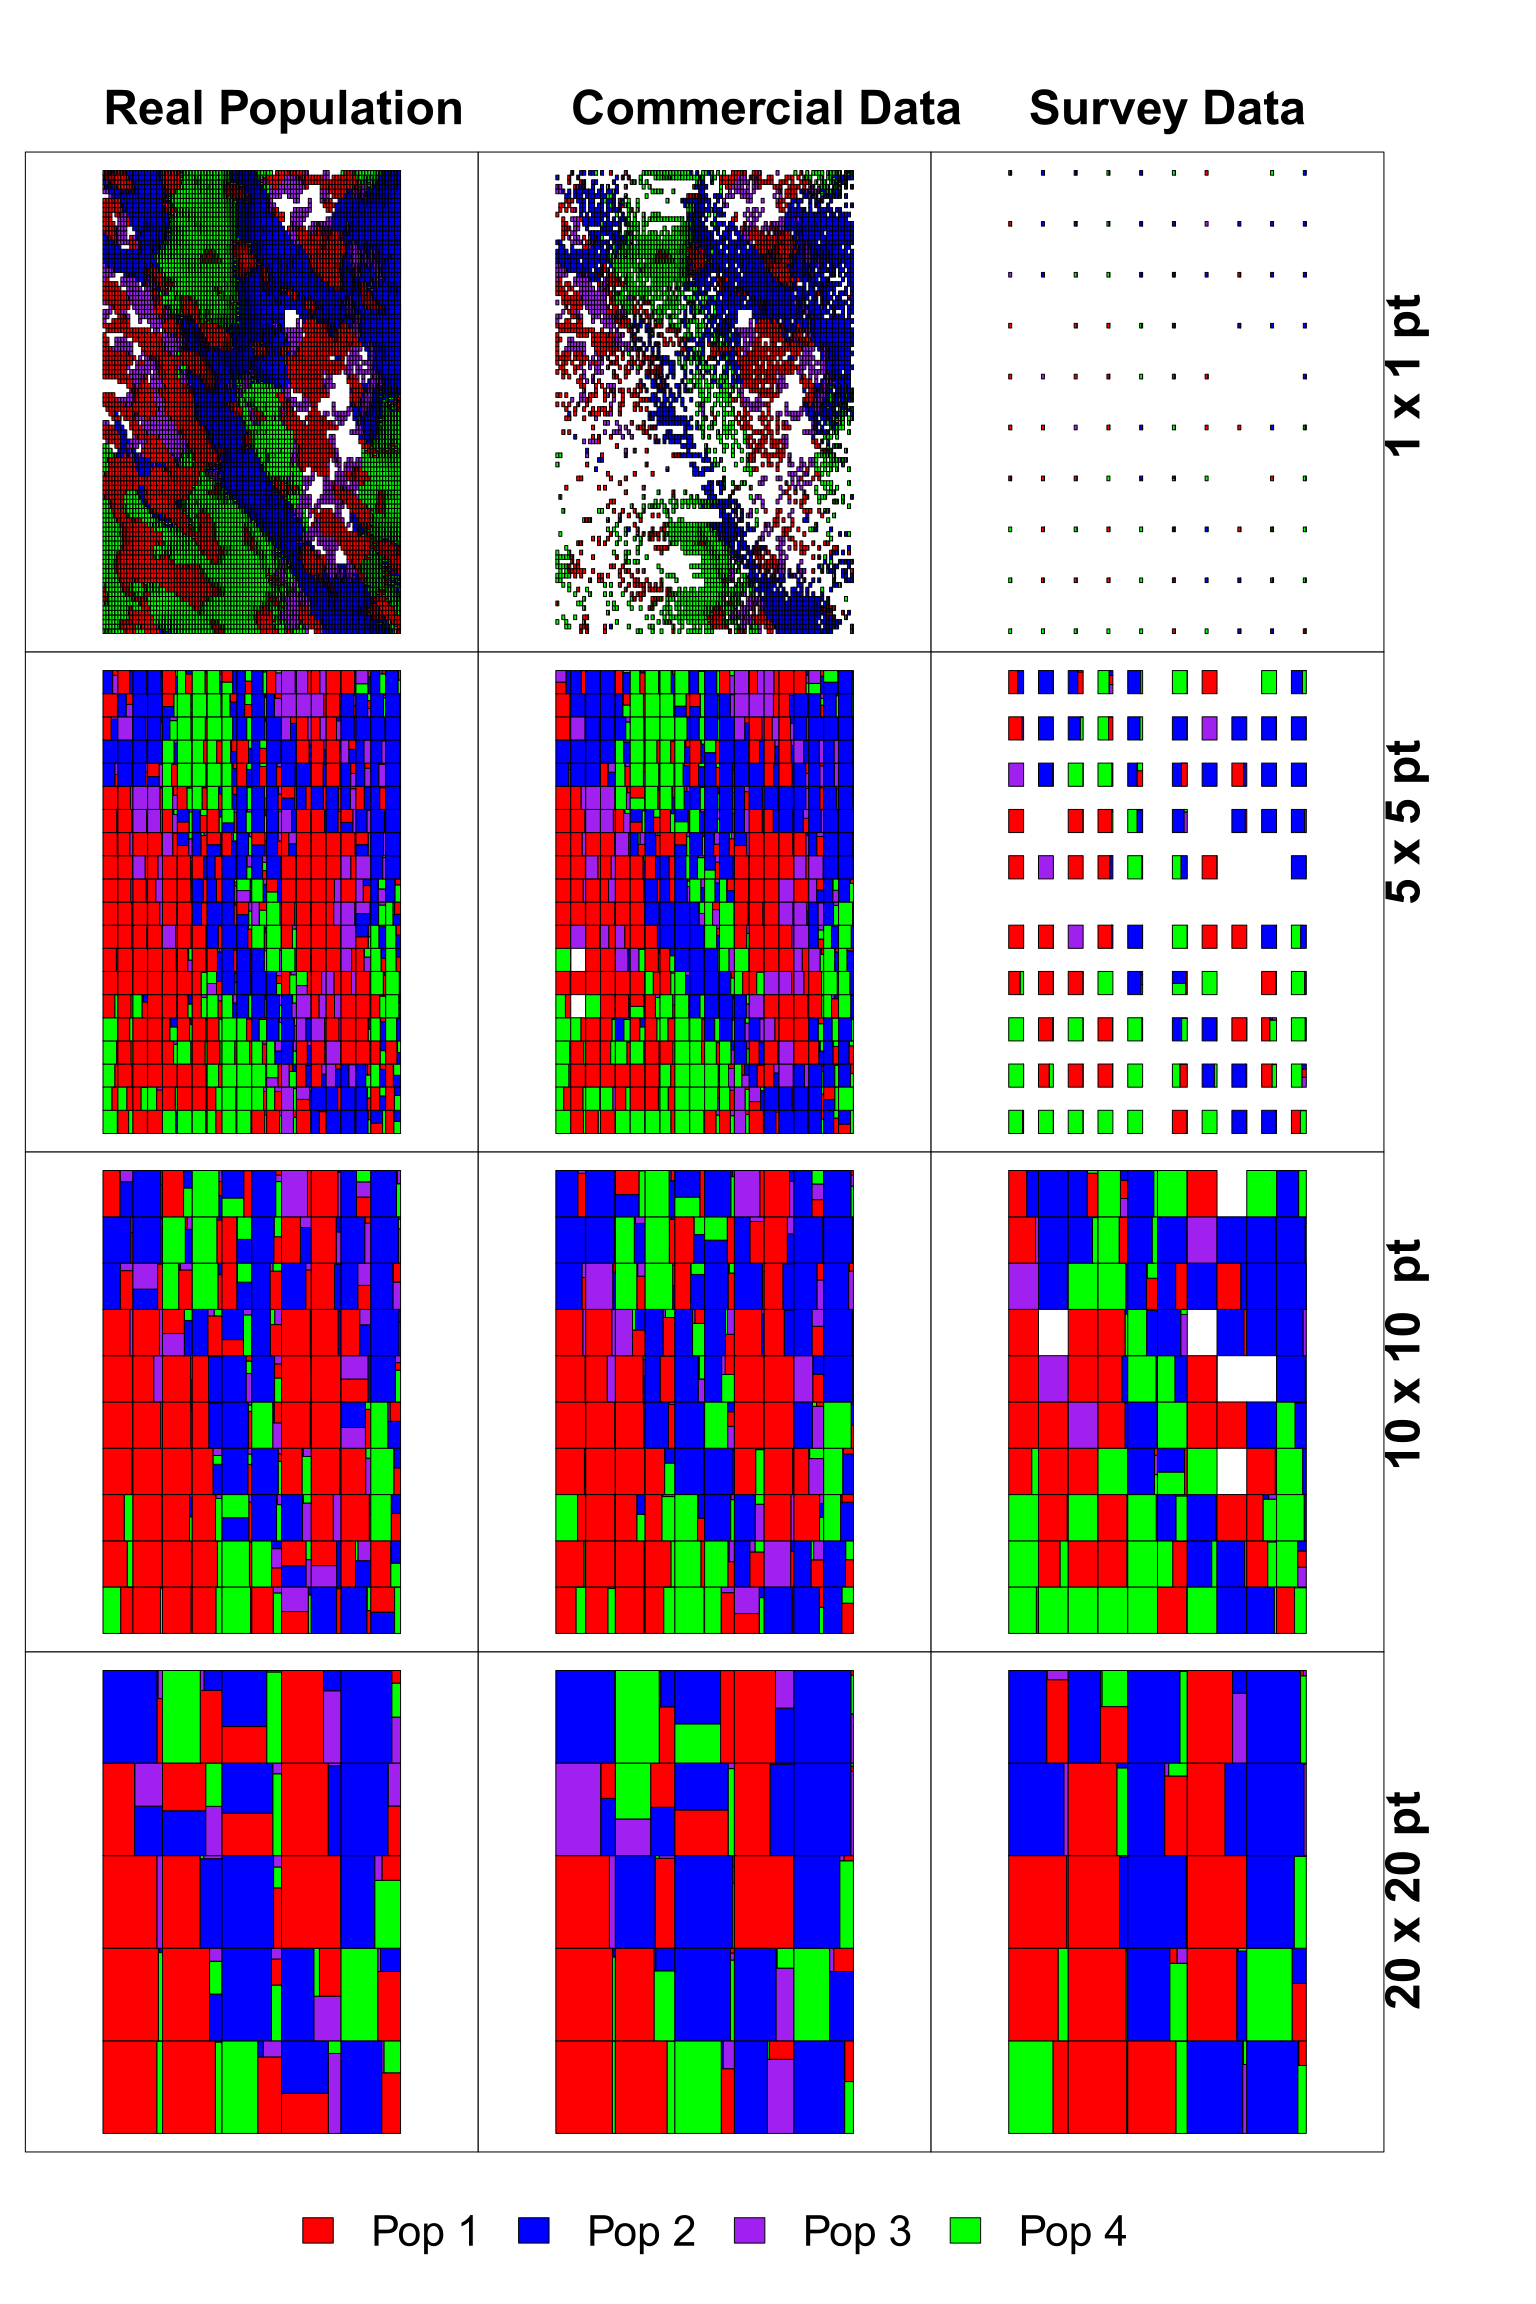
\includegraphics[width =\linewidth]{../analysis/Data_Aggregation_space}
	\caption{Data aggregation at different spatial resolutions over a
		ten year period}
	\label{fig:1}
\end{figure}	

\begin{figure}[!ht]
	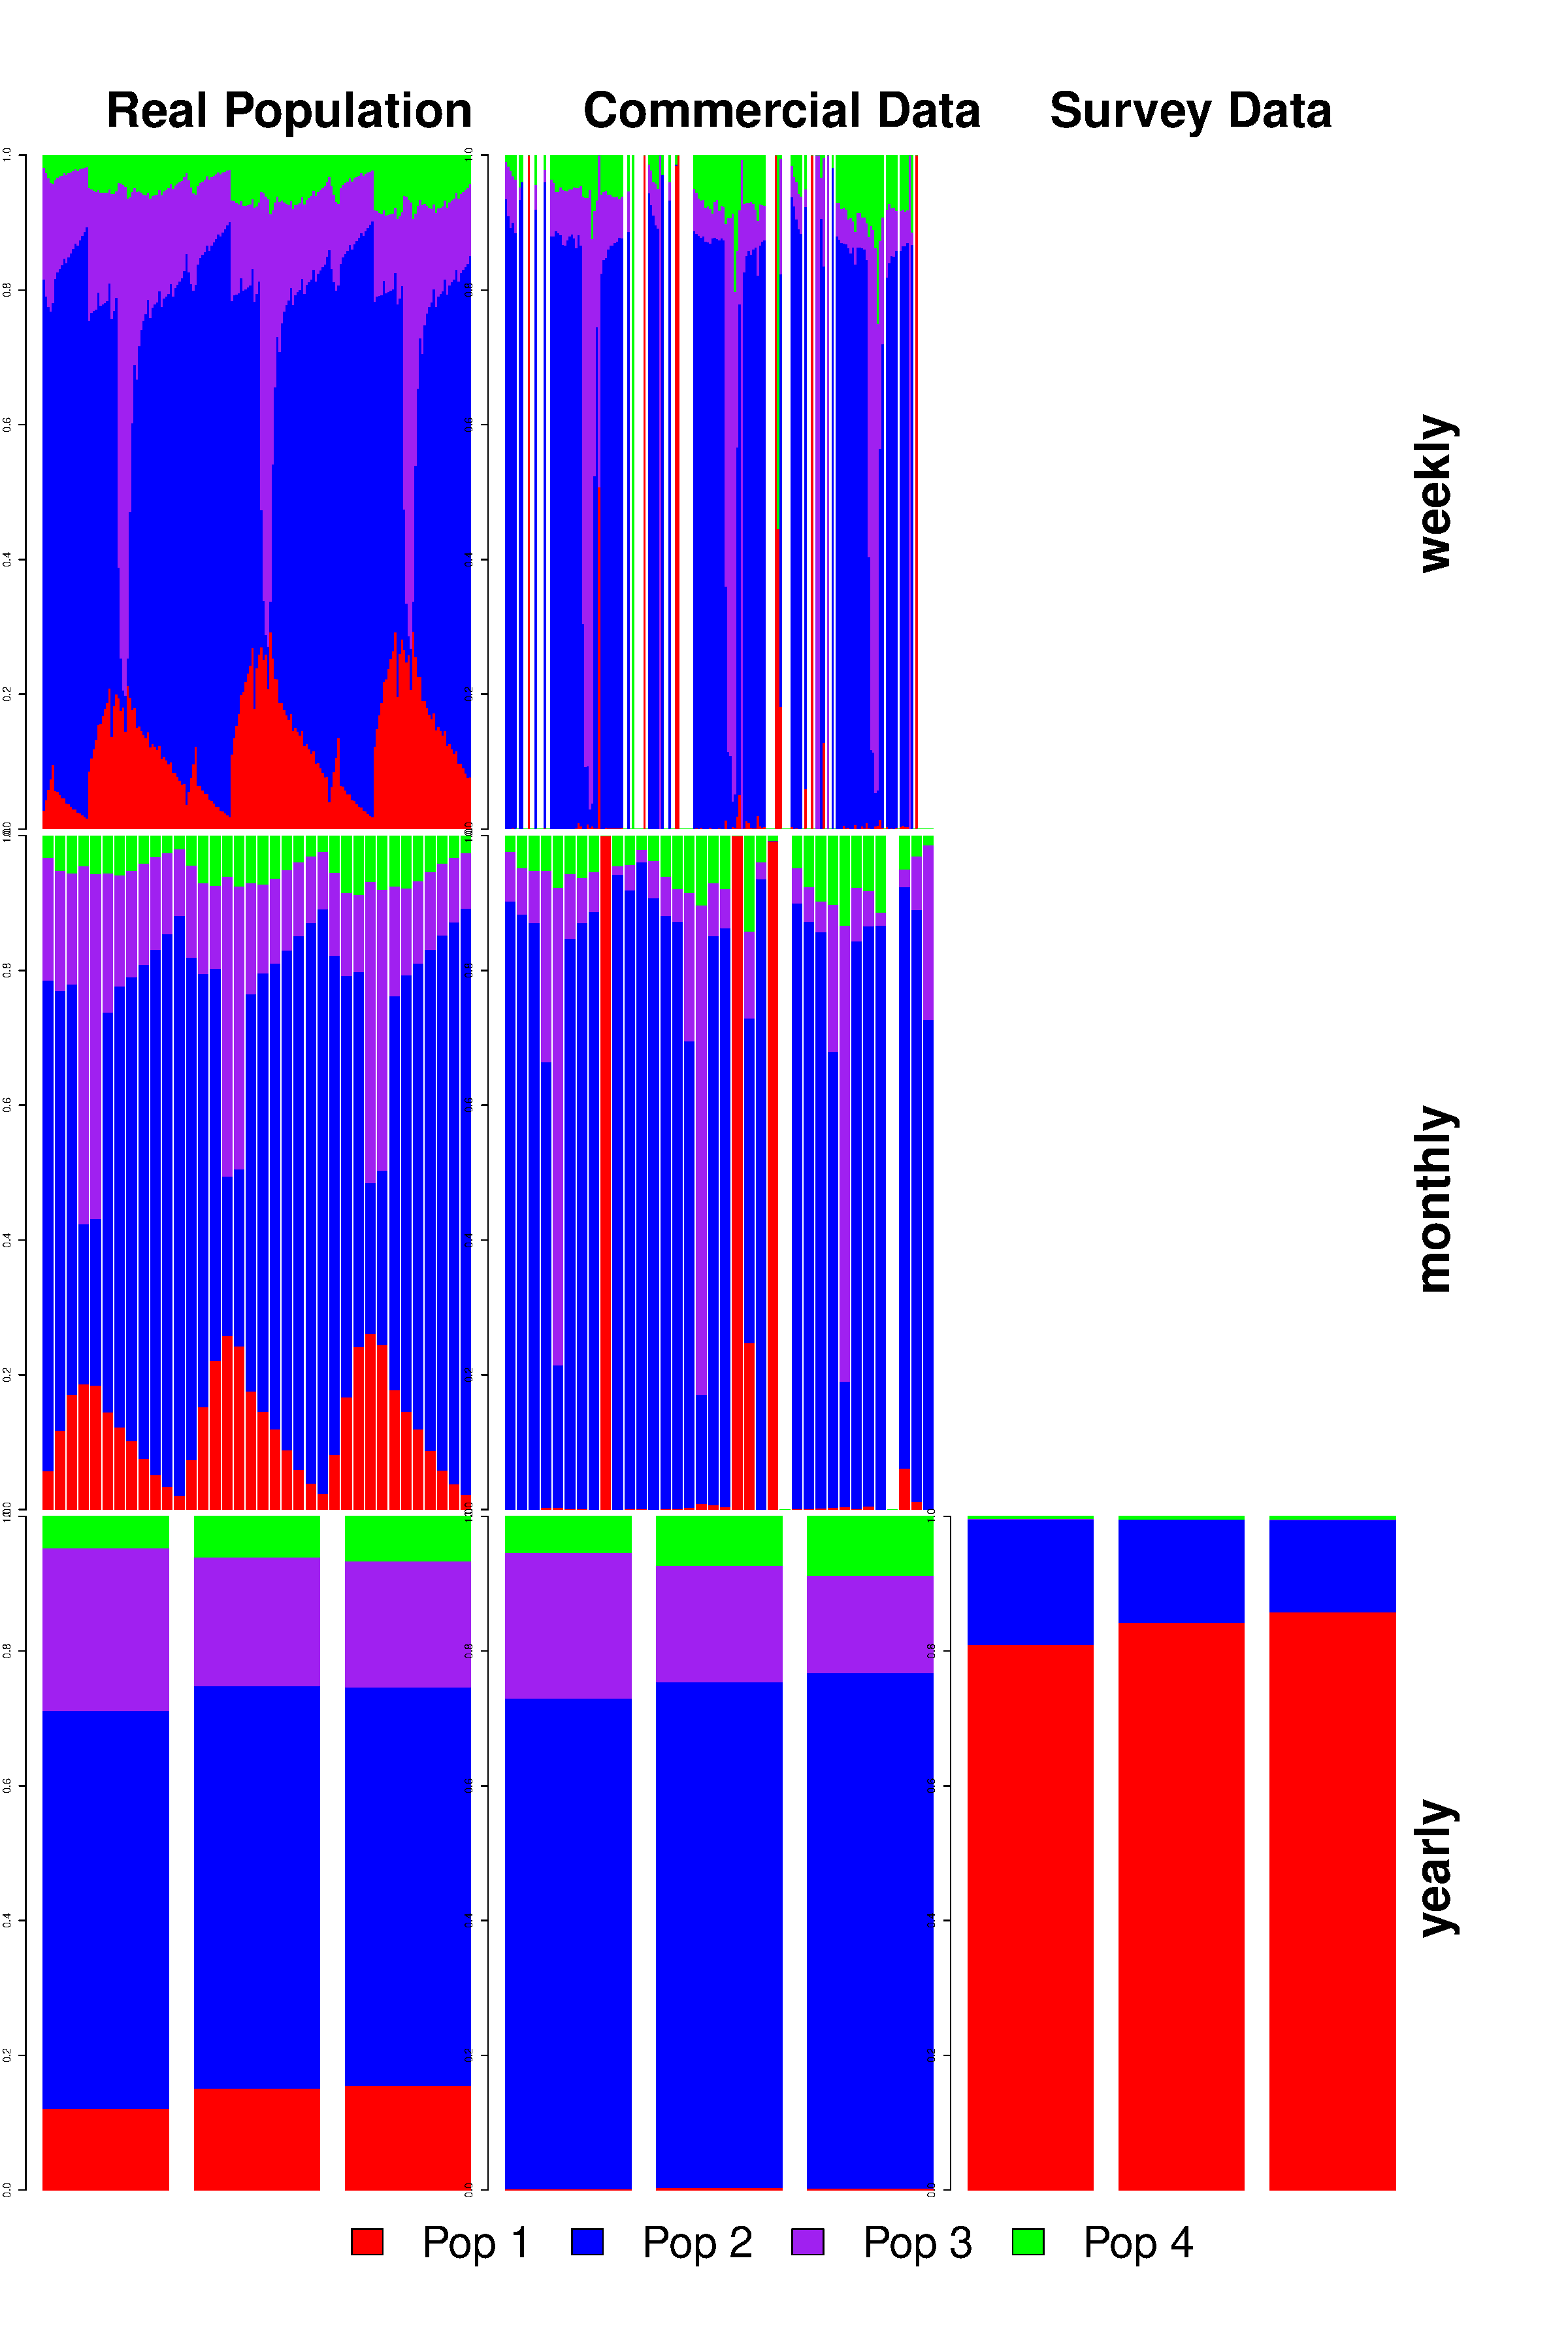
\includegraphics[width = \linewidth]{../analysis/Data_Aggregation_time}
	\caption{Data aggregation at different temporal resolutions over a
		three year period}
	\label{fig:2}
\end{figure}	


\begin{figure}[!ht]
	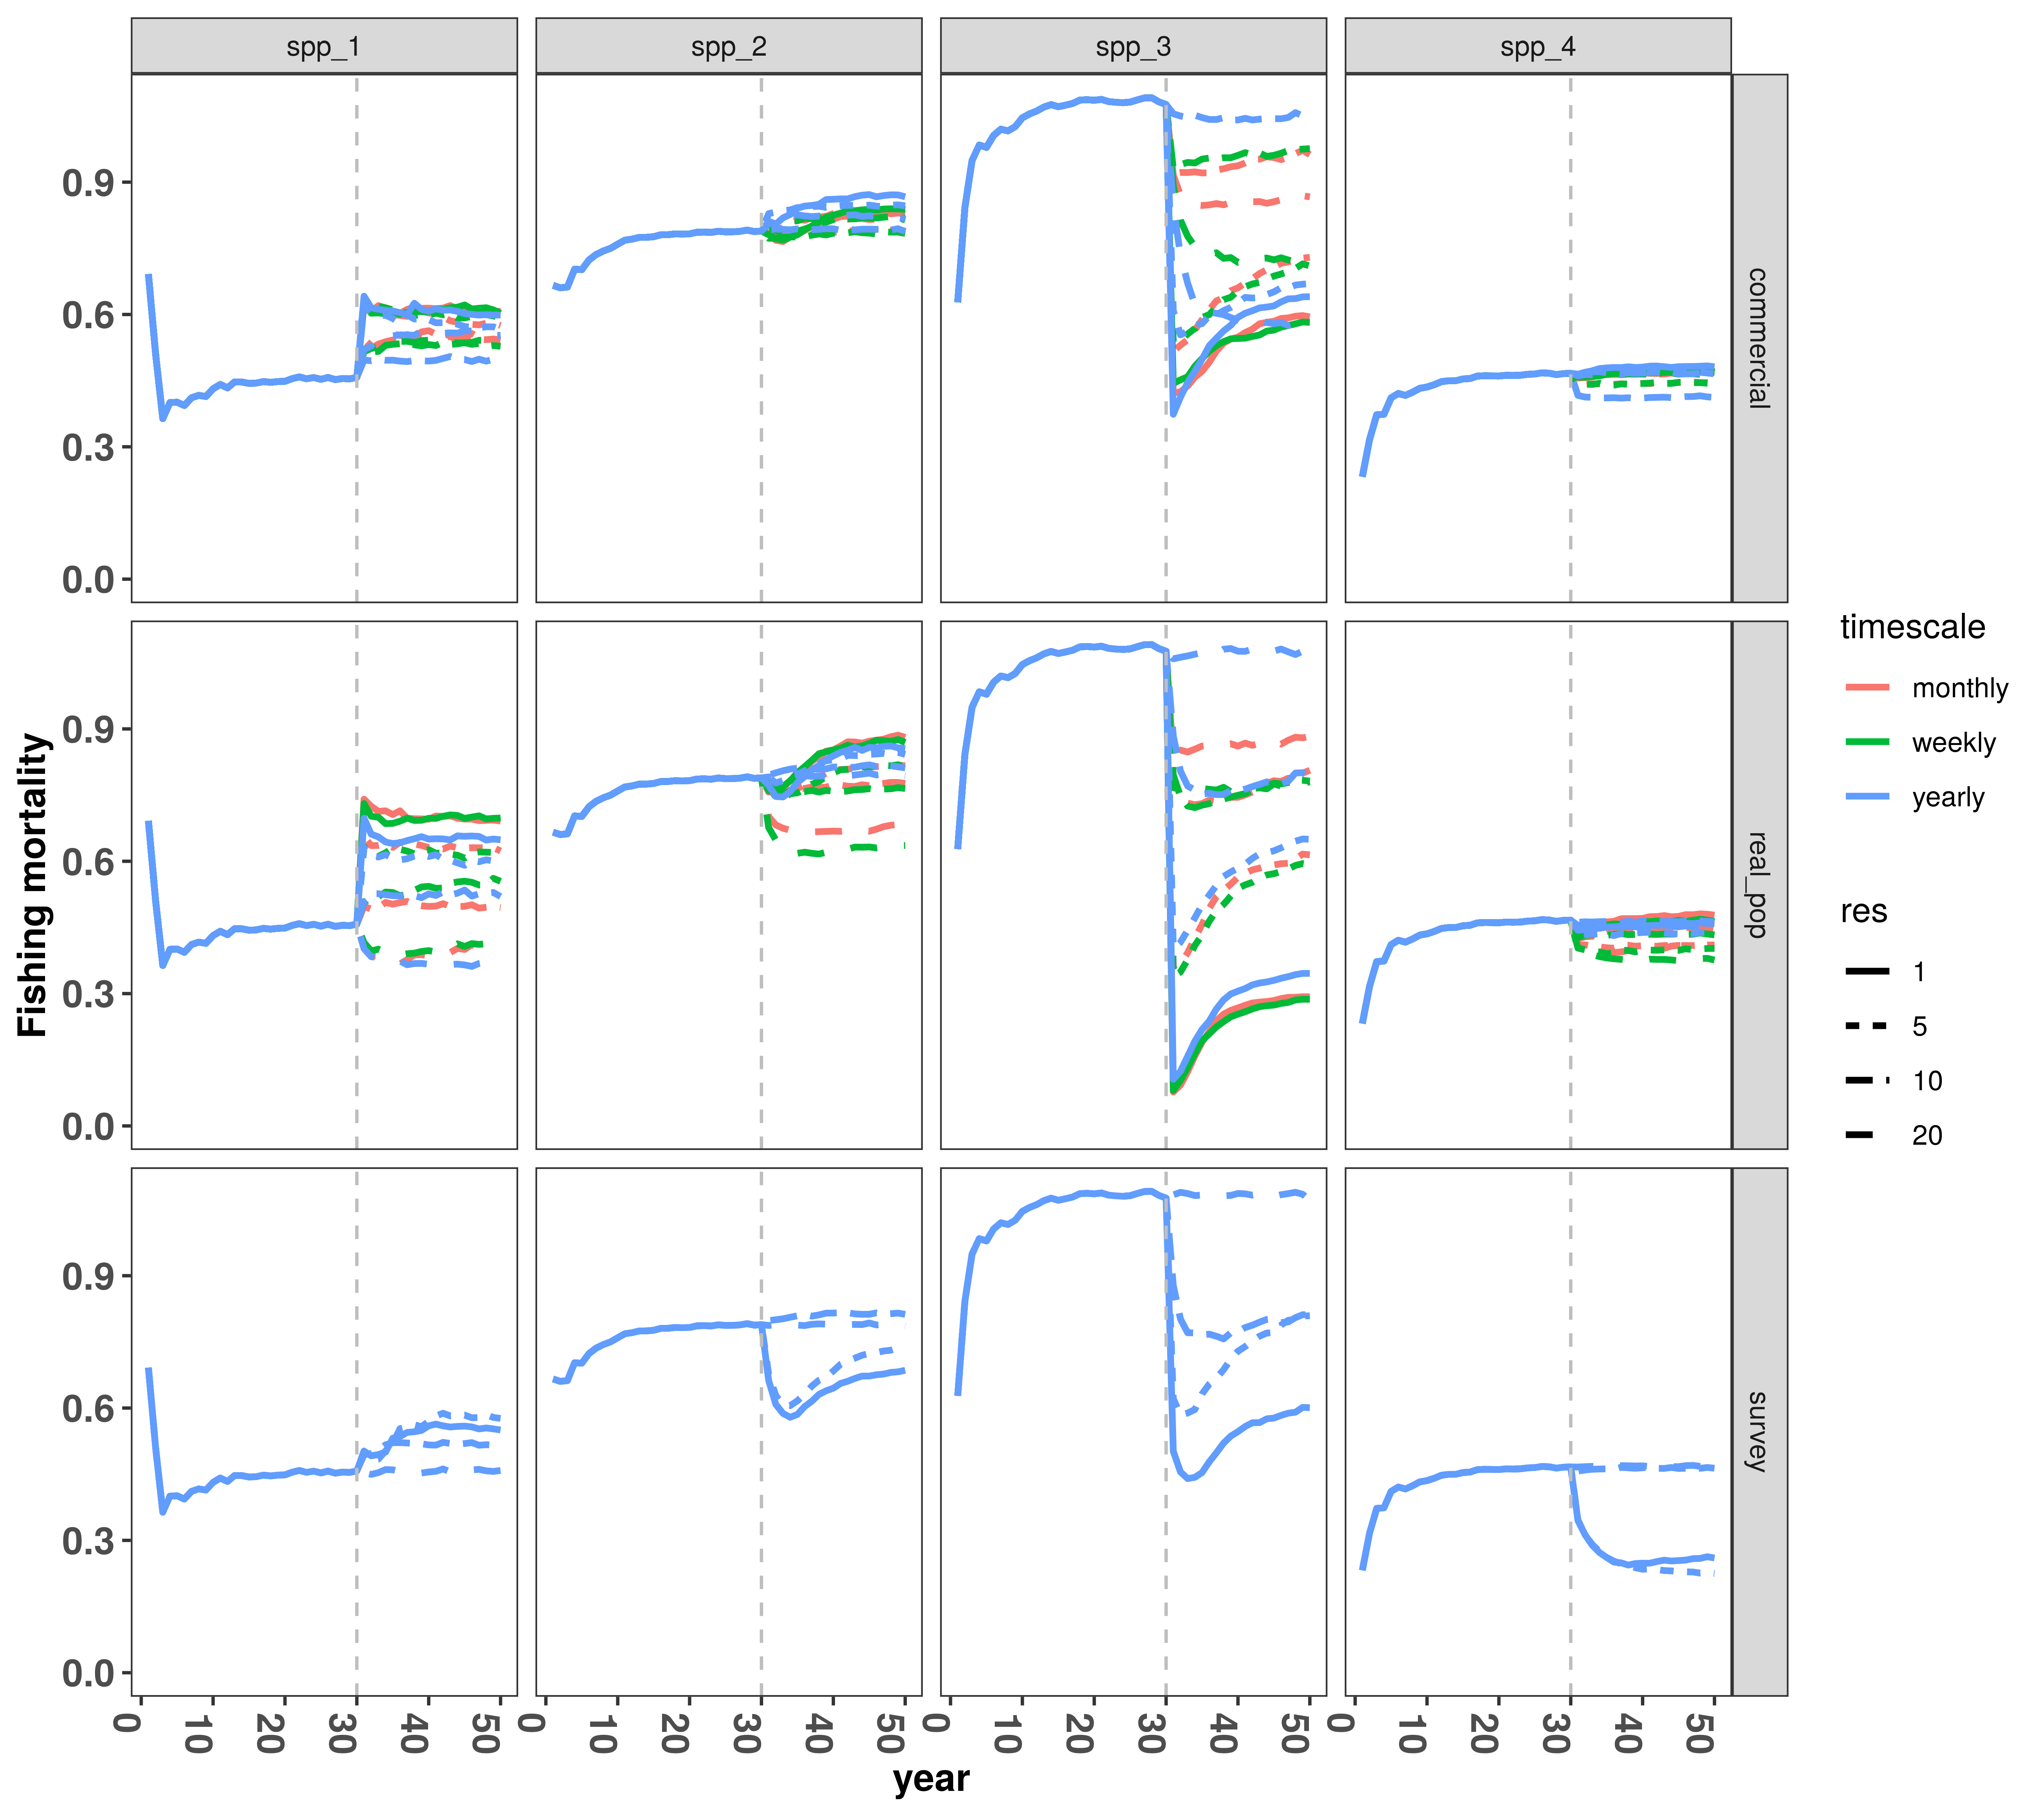
\includegraphics[width = \linewidth]{../analysis/F_trendsREV}
	\caption{Comparison of closure scenarios - Fishing mortality trends.
		Only the scenarios based on high catch rates of population 3
		are shown.}
	\label{fig:3}
\end{figure}

\begin{figure}[!ht]
	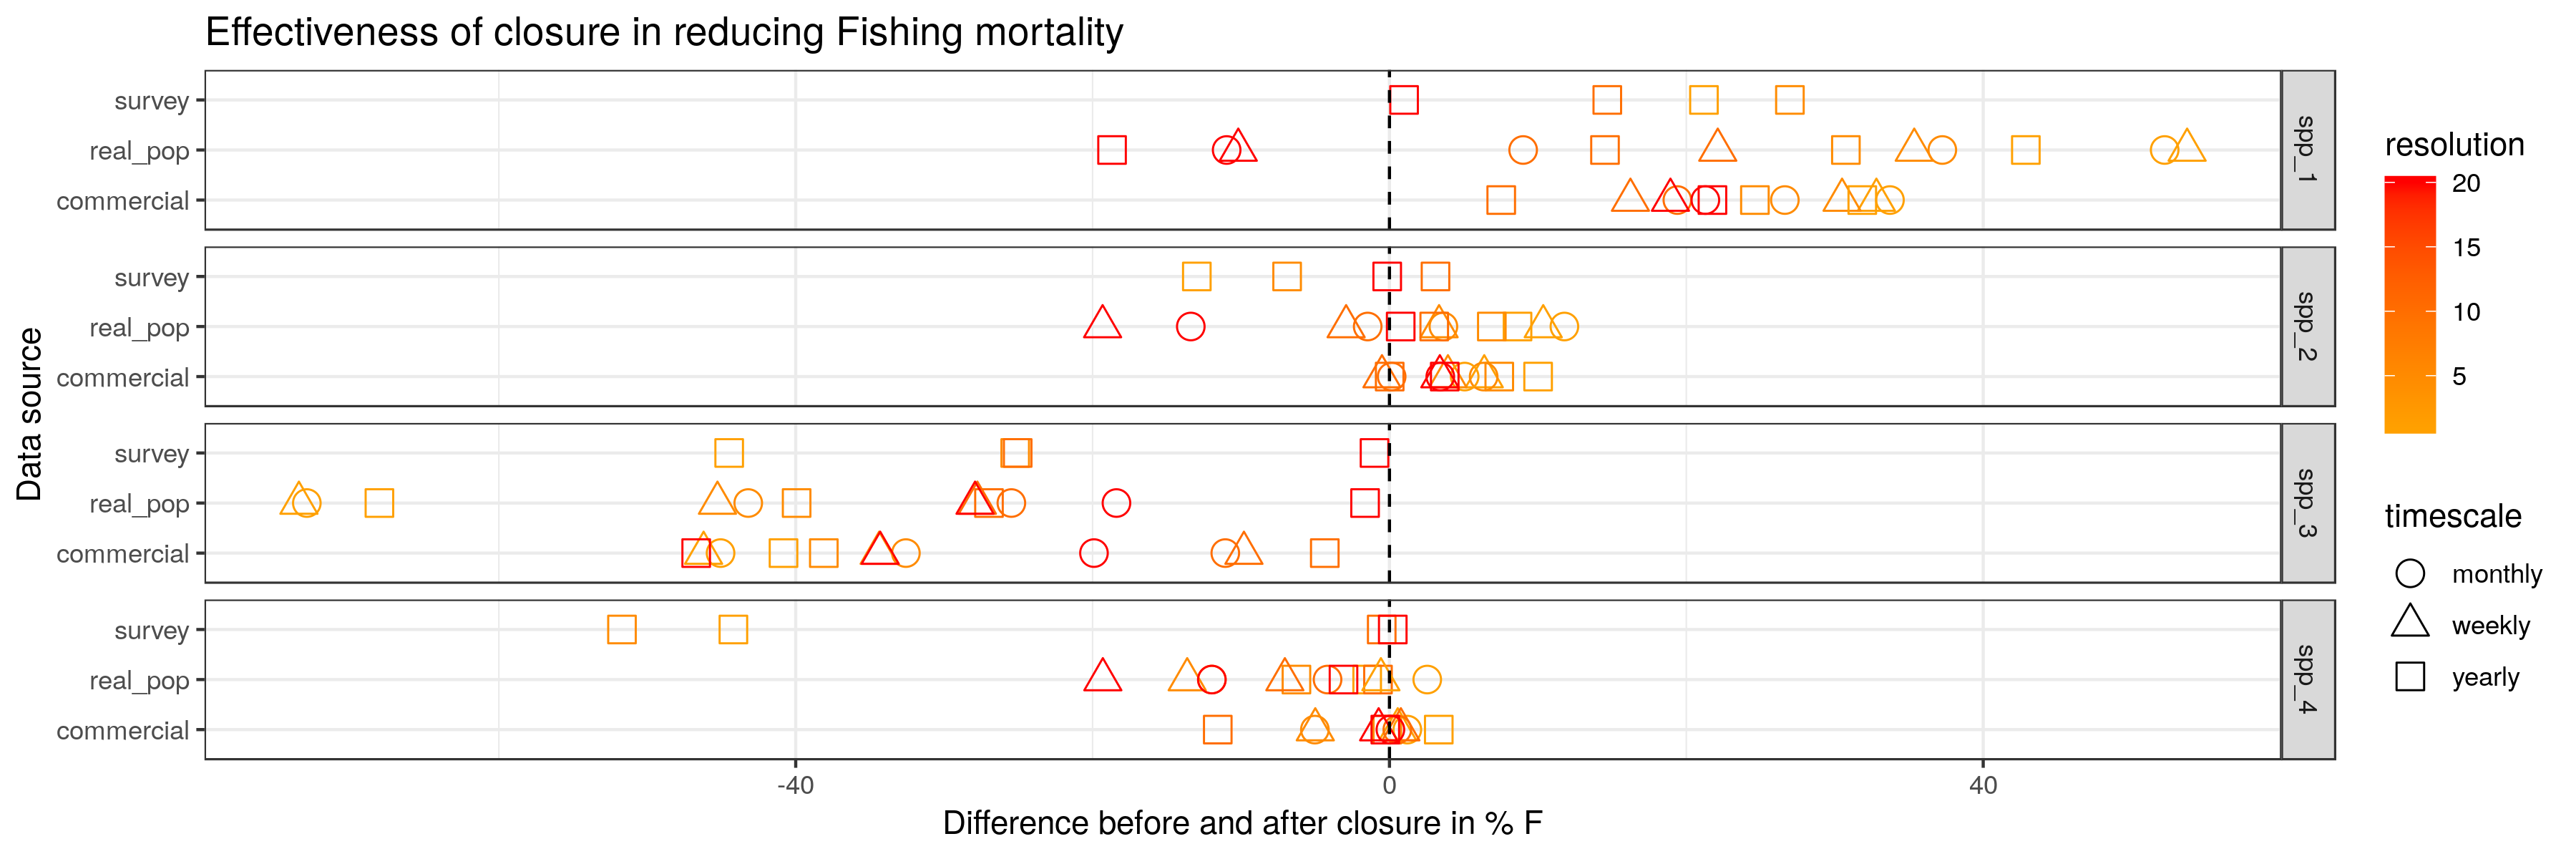
\includegraphics[width =\linewidth]{../analysis/Overview_plot_highPopRev}
	\caption{Comparison of closure scenarios. Points indicate the
		difference between the fishing mortality pre-closure (year 29)
		and post-closure (year 50) for population 3. Only the scenarios
		based on high catch rates of population 3 are shown.}
	\label{fig:4}
\end{figure}	

\clearpage

\section*{References}

\bibliography{simulation_framework}

\end{document}
